\documentclass[9pt]{beamer}

\mode<presentation> 
{ %\usetheme[nat,dogma]{Frederiksberg} }
  \usetheme{Diku}
}

\usepackage{manfnt}
% \usepackage[danish]{babel}
\usepackage[latin1]{inputenc}
\usepackage{times}
\usepackage[T1]{fontenc}
\usepackage[polutonikogreek,english]{babel}
\usepackage{hyperref}
\usepackage{animate}
%\usepackage{multimedia}
\usepackage{francois-preamble}
\usepackage{multirow}
\usepackage{tikz}
\usetikzlibrary{shapes,arrows}
\usetikzlibrary{arrows,decorations.pathmorphing,backgrounds,fit,positioning,shapes.symbols,chains}
%\usepackage{movie15}
\usepackage{tcolorbox}
\newcommand<>{\tmpbox}[1]{
    \definecolor{colorbox}{RGB}{255,255,255}
    \only#2{%
      \definecolor{colorbox}{RGB}{5,61,245}%
    }
    \tcbox[opacityback=1,opacityframe=0.5,colframe=colorbox,nobeforeafter,tcbox raise base,left=-1.5mm,right=-1.5mm]{#1}
}




\newcommand{\cc}{{c\!\!,}}
\newcommand{\degr}[1]{{{#1}^\circ}}


\newcommand{\phos}
{%
\selectlanguage{polutonikogreek}%
f~ws/fwt'os
\selectlanguage{english}%
}


\newcommand{\metron}
{%
\selectlanguage{polutonikogreek}%
m'etron
\selectlanguage{english}%
}


\newcommand{\stereos}
{%
\selectlanguage{polutonikogreek}%
stere'os
\selectlanguage{english}%
}



\title{Vision and Image Processing:\\ Shading, Photometric Stereo}

\author[F.~Lauze] % (optional, use only with lots of authors)
{Fran{\c c}ois Lauze}

\institute[DIKU] % (optional, but mostly needed)
{
  Department of Computer Science\\
  University of Copenhagen
}

\date[2019-20 B2] % (optional, should be abbreviation of conference name)
% {Research Presentation, Diku 2006}

\definecolor{gold}{rgb}{0.95,0.83,0.0}
\definecolor{orange}{rgb}{0.95,0.7,0.0}
% \definecolor{backblue}{rgb}{0.93,0.94,0.99}
\definecolor{backblue}{rgb}{0.95,0.94,0.99}
\setbeamercolor*{background canvas}{bg=backblue} 



\newcommand{\myemph}[1]{{\color{blue}{#1}}}
\newcommand{\intrg}[1]{\int_{{#1}=-\infty}^\infty}
\newcommand{\intRR}{\int_{-\infty}^\infty}

\AtBeginSection[]
{
  \begin{frame}<beamer>{Outline}
    \tableofcontents[currentsection,currentsubsection]
  \end{frame}
}

\begin{document}
\maketitle

% would be cool with more images showing applications


%-------------------------------------------------------------------
%   Start slides
%-------------------------------------------------------------------




%----------------------------------------------



\begin{frame}
  \frametitle{Plan for today and December 4th}
  \begin{itemize}
  \item Image Formation and reflectance.
  \item Lighting Models.
  \item The Photometric Stereo Problem.
  \end{itemize}
\end{frame}


\section{What is Photometric Stereo}


\begin{frame}
  \frametitle{The Photometric Stereo (PS) Problem [Woodham, 1980]}
  \begin{columns}
    \begin{column}{0.5\textwidth}
      \begin{center}
        \fbox{
          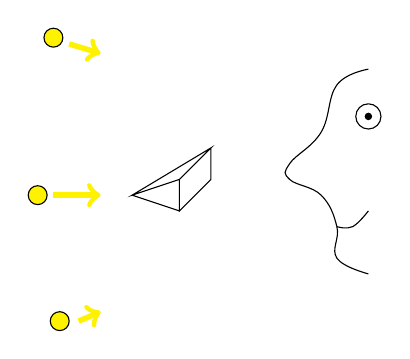
\begin{tikzpicture}[scale=0.4]
% La camera
\path[draw] (-0.5,0)--(1,-0.5)--(1,0.5)--(-0.5,0)--(2,1.5)--(1,0.5)--(1,-0.5)--(2,0.5)--(2,1.5);

% Les trois soleils
\uncover<2->{
\draw[fill=yellow] (-3,5) circle(0.3);
\draw[->,line width=2pt, yellow] (-2.5,4.8)--(-1.5,4.5);
}
\uncover<3->{
\draw[fill=yellow] (-3.5,0) circle(0.3);
\draw[->,line width=2pt, yellow] (-3,0)--(-1.5,0);
}
\uncover<4->{
\draw[fill=yellow] (-2.8,-4) circle(0.3);
\draw[->,line width=2pt, yellow] (-2.2,-4)--(-1.5,-3.7);
}



% Contour d'une tete
\draw  plot[smooth, tension=.7] coordinates {(7,4) (6,3.5) (5.5,2) (4.5,1) (4.5,0.5) (5.5,0) (6,-1) (6,-2) (7,-2.5)};
% Yeux
\draw (7,2.5) circle(0.4);
\draw[fill] (7,2.5) circle(0.1);
% Bouche
\draw  plot[smooth, tension=.7] coordinates {(6,-1) (6.5,-1) (7,-0.5)};

\end{tikzpicture}
        }
      \end{center}  
    \end{column}
    \begin{column}{0.5\textwidth}
      \begin{itemize}
      \item $1$ \myemph{fixed camera} + $1$ ``fixed'' scene
      \item $m$ lightings
      \end{itemize}
      \begin{block}{Goal:}<5>
        {3D-reconstruction} of the scene from the 2D images
      \end{block}
    \end{column}
  \end{columns}
  \begin{columns}
    \begin{column}{0.22\textwidth}
      \begin{center} 
        \uncover<2->{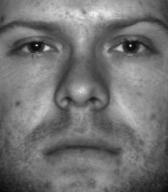
\includegraphics[width=0.9\textwidth]{FIGURES/Face01_1}}
      \end{center}
    \end{column}
    \begin{column}{0.22\textwidth}
      \begin{center}
        \uncover<3->{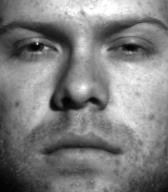
\includegraphics[width=0.9\textwidth]{FIGURES/Face01_2}}
      \end{center}
    \end{column}
    \begin{column}{0.22\textwidth}
      \begin{center}
        \uncover<4->{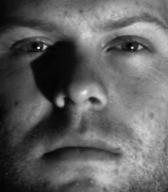
\includegraphics[width=0.9\textwidth]{FIGURES/Face01_3}}
      \end{center}
    \end{column} 
    \begin{column}{0.22\textwidth}
      \begin{center}
        \uncover<5->{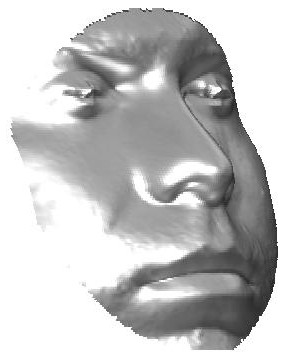
\includegraphics[width=0.9\textwidth]{FIGURES/Face01_shape}}
      \end{center}
    \end{column}  
  \end{columns} 
  {\fontsize{5}{5}\selectfont Slide by Y. Qu{\'e}au}
\end{frame}



\begin{frame}[t]{Ingredients for Photometric Stereo}
  \begin{center}
    \huge
    \tmpbox<2>{Photo}\hspace{-5.5mm}\tmpbox<3>{metric} \tmpbox<4>{Stereo}
  \end{center}
  \begin{itemize}
  \item \onslide<2->{\phos: (ph\~os, gen. phot\'os): light}
  \item \onslide<3->{\metron (m\'etron): measure}
  \item \onslide<4->{\stereos (stere\'os): solid/volume}
  \end{itemize}
  \vfill
  \pause
  \onslide<5->{Suggest. Volume recovery from measured light. Needed:~\\~\\}
  \onslide<6->{
    \begin{itemize}
    \item Understand reflectance: how is light reflected from an object.
    \item How can we measure it.
    \item How object geometry is linked to light.
    \end{itemize}
  }
\end{frame}


\section{Lighting Models}


\begin{frame}[t]{Light and Image Formation}
  \begin{columns}
    \begin{column}{0.5\textwidth}
      \begin{center}
          \only<1>{\includegraphics[width=0.9\textwidth]{FIGURES/imform_obj}}
          \only<2>{\includegraphics[width=0.9\textwidth]{FIGURES/imform_obj_cam}}
          \only<3>{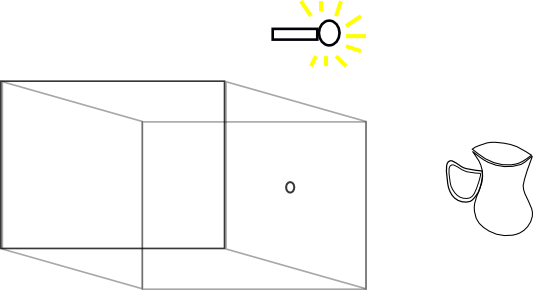
\includegraphics[width=0.9\textwidth]{FIGURES/imform_obj_cam_light}}
          \only<4->{\includegraphics[width=0.9\textwidth]{FIGURES/imform}}
      \end{center}
    \end{column}
    \begin{column}{0.5\textwidth}
      \begin{block}{Ingredients}
        \begin{itemize}[<+->]
        \item Object
        \item Camera
        \item Light source
        \item Light reflection by object surface.
        \end{itemize}
      \end{block}
    \end{column}
  \end{columns}
  ~\vspace{0.5cm}\\
  \begin{itemize}[<+->]
  \item Image formation inside camera: when light, scene and camera parameters known: reflectance function.
  \item BTW: Camera detectors react almost truly linearly to received luminance. \pause
  \item Can image formation model give enough information about the object surface to reconstruct it?
  \end{itemize}
\end{frame}



\begin{frame}[t]{Materials and Light}
  \begin{center}
   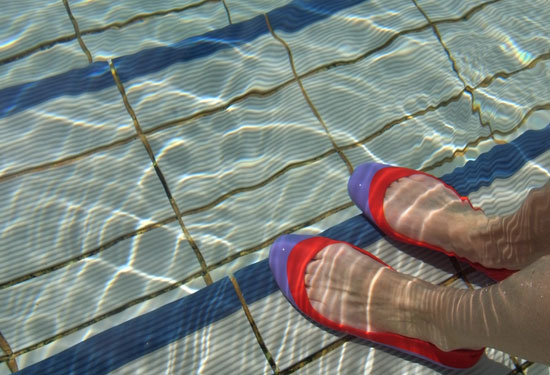
\includegraphics[width=0.8\textwidth]{FIGURES/transparent_and_opaque}
  \end{center}
  ~\\
  \pause
  From now, only opaque objects.
\end{frame}


\begin{frame}[t]{Matte vs Brilliant}
  \begin{center}
   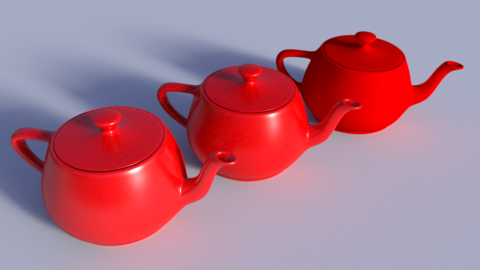
\includegraphics[width=0.8\textwidth]{FIGURES/TeaPotShading}
  \end{center}
  ~\\
\end{frame}


\begin{frame}{Bidirectional Reflectance Distribution Function -- BRDF}
  \begin{columns}
    \begin{column}{0.6\textwidth}
      \begin{center}
        \only<1>{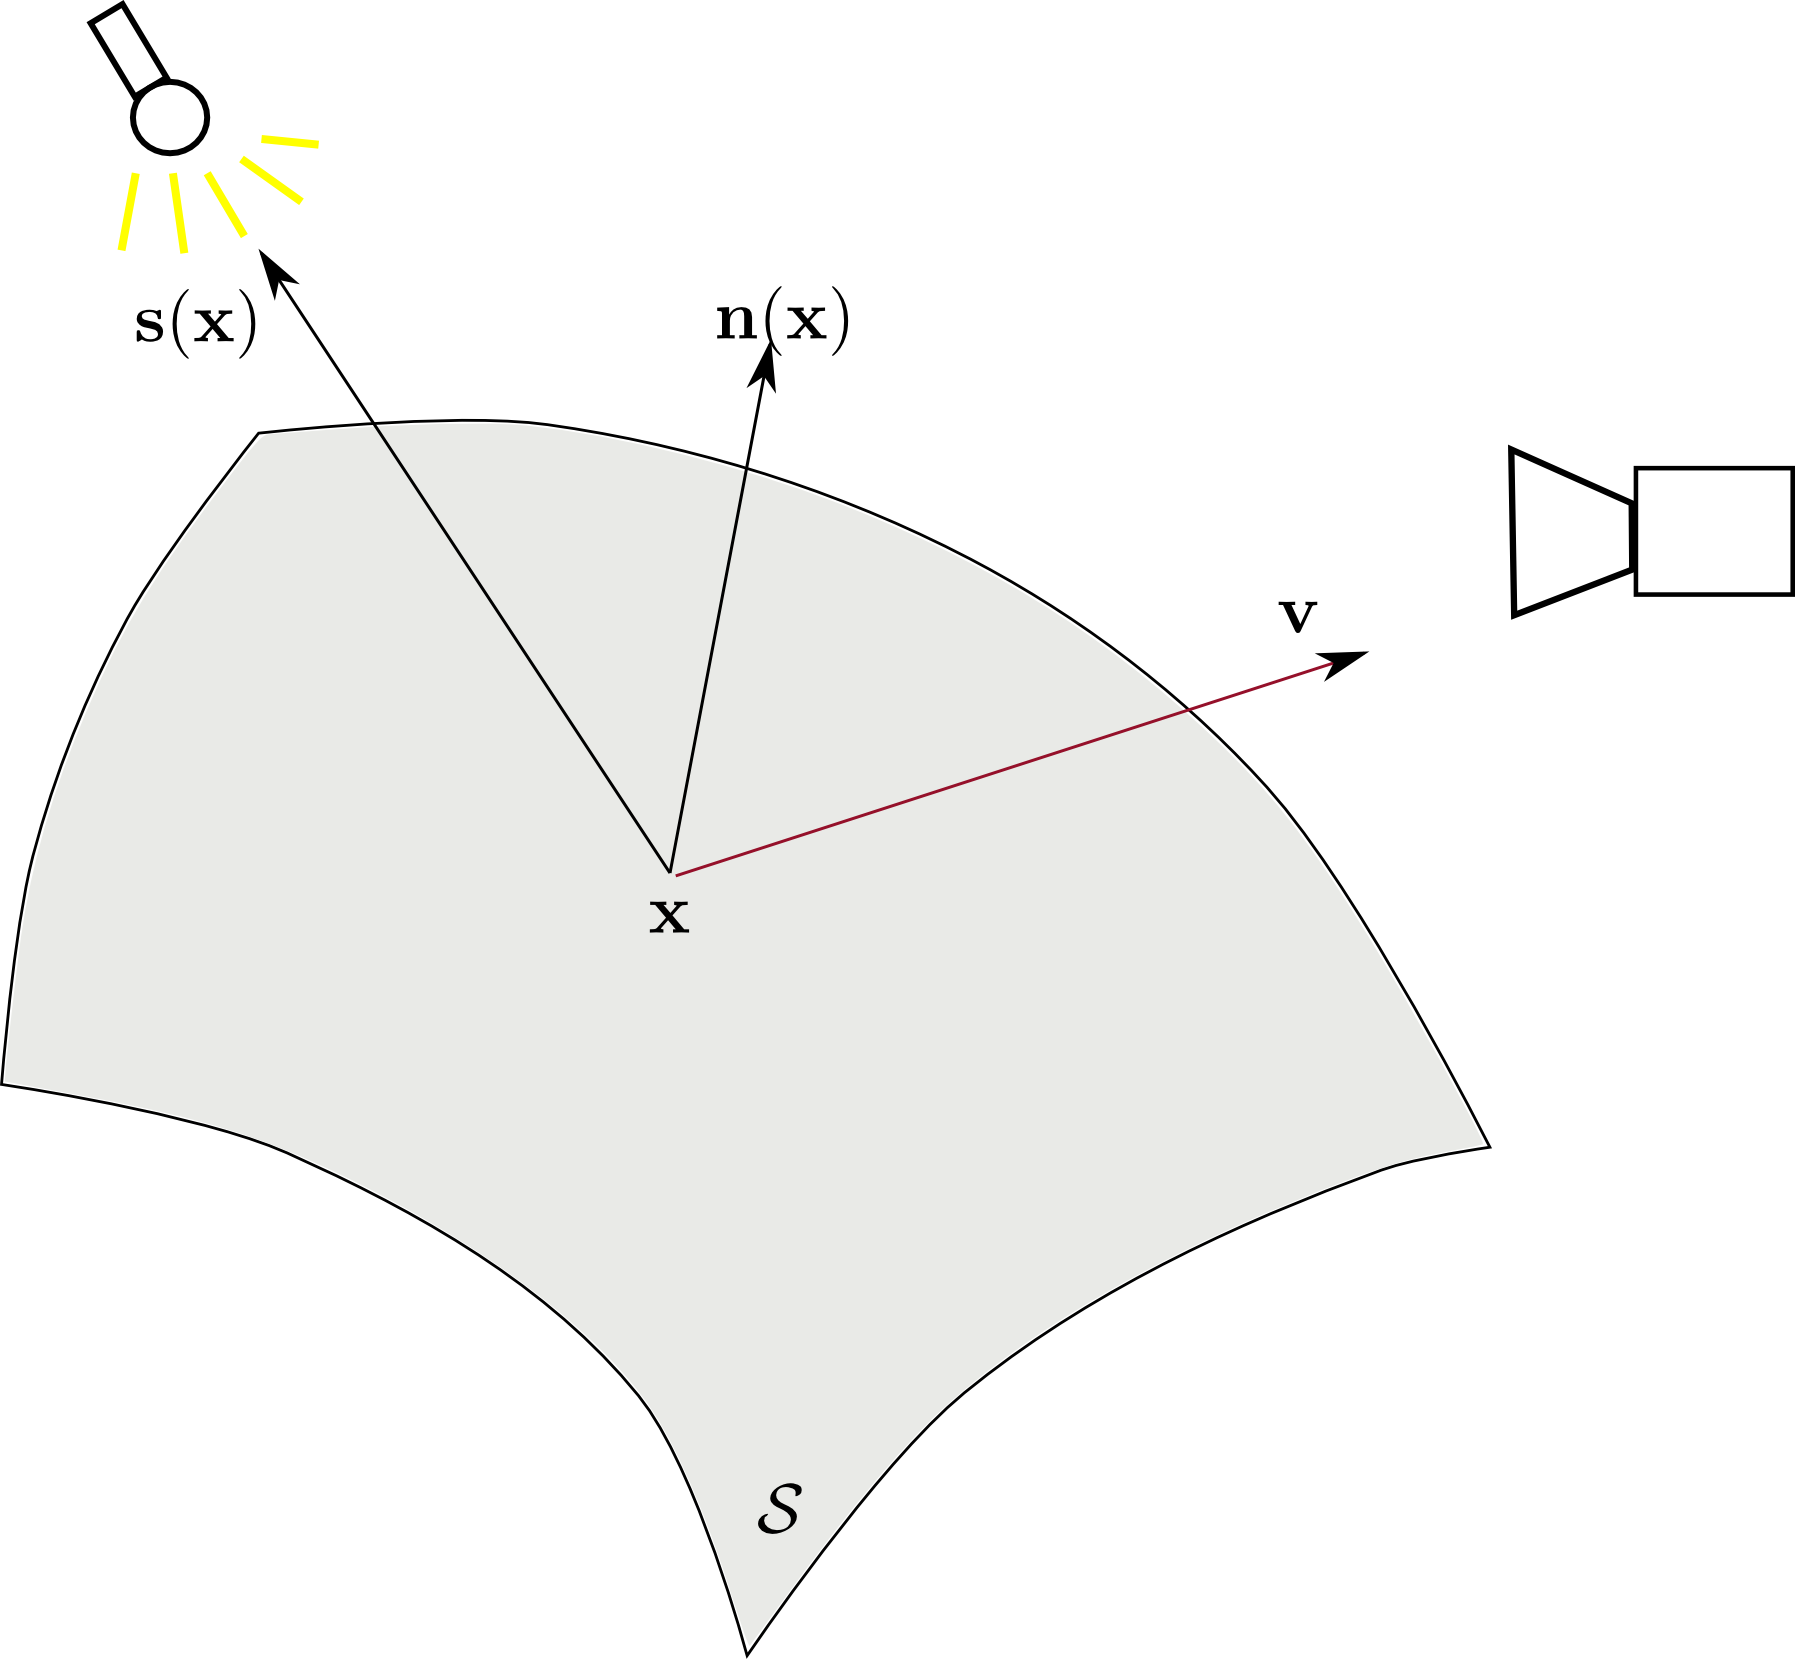
\includegraphics[width=0.75\textwidth]{FIGURES/reflectance}}
        \only<2->{
\includegraphics[width=0.75\textwidth]{FIGURES/reflectance2}}
      \end{center}
    \end{column}
    \pause
    \begin{column}{0.4\textwidth}
      \only<3->{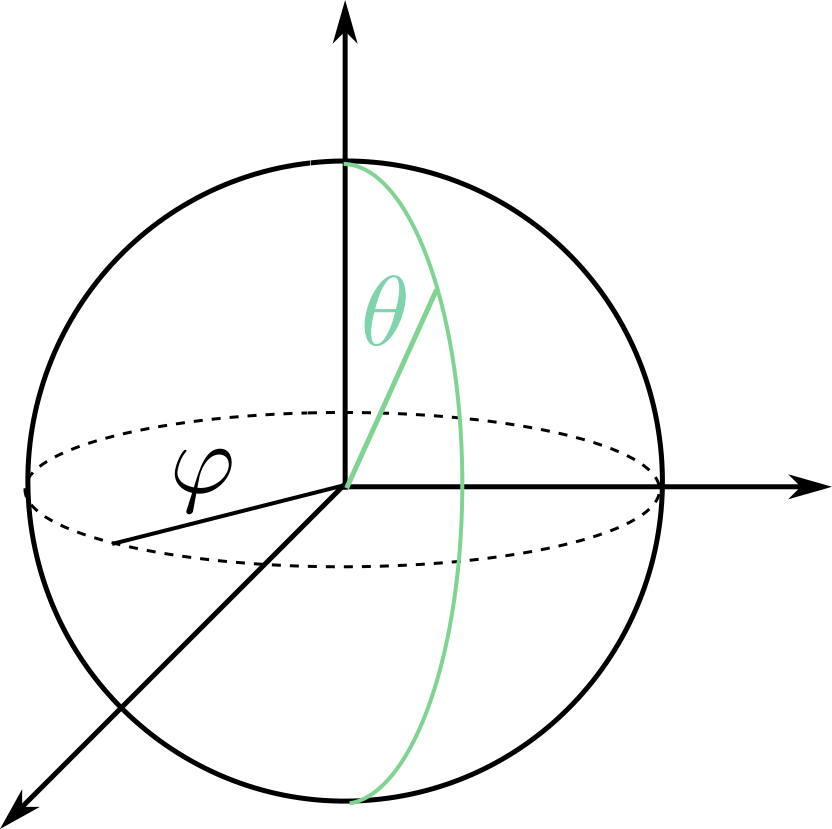
\includegraphics[width=0.5\textwidth]{FIGURES/spherical_coordinates}}
    \end{column}
  \end{columns}
  \pause
  \begin{itemize}
  \item $E^s(\bx,\theta_i,\phi_i)$: \emph{Irradiance} at surface (at pos $\bx$) in direction $\theta_i,\phi_i$
  \item $L^s(\bx,\theta_e,\phi_e)$: \emph{Radiance} at surface (at pos $\bx$) in direction $\theta_e,\phi_e$
  \end{itemize}
$$\kappa(\bx,\theta_i,\phi_i,\theta_e,\phi_e) = \frac{L^s(\bx,\theta_e,\phi_e)}{E^s(\bx,\theta_i,\phi_i)}$$
\end{frame}



\begin{frame}[t]{Bidirectional Reflectance Distribution Function -- BRDF}
  \begin{center}
    \only<1>{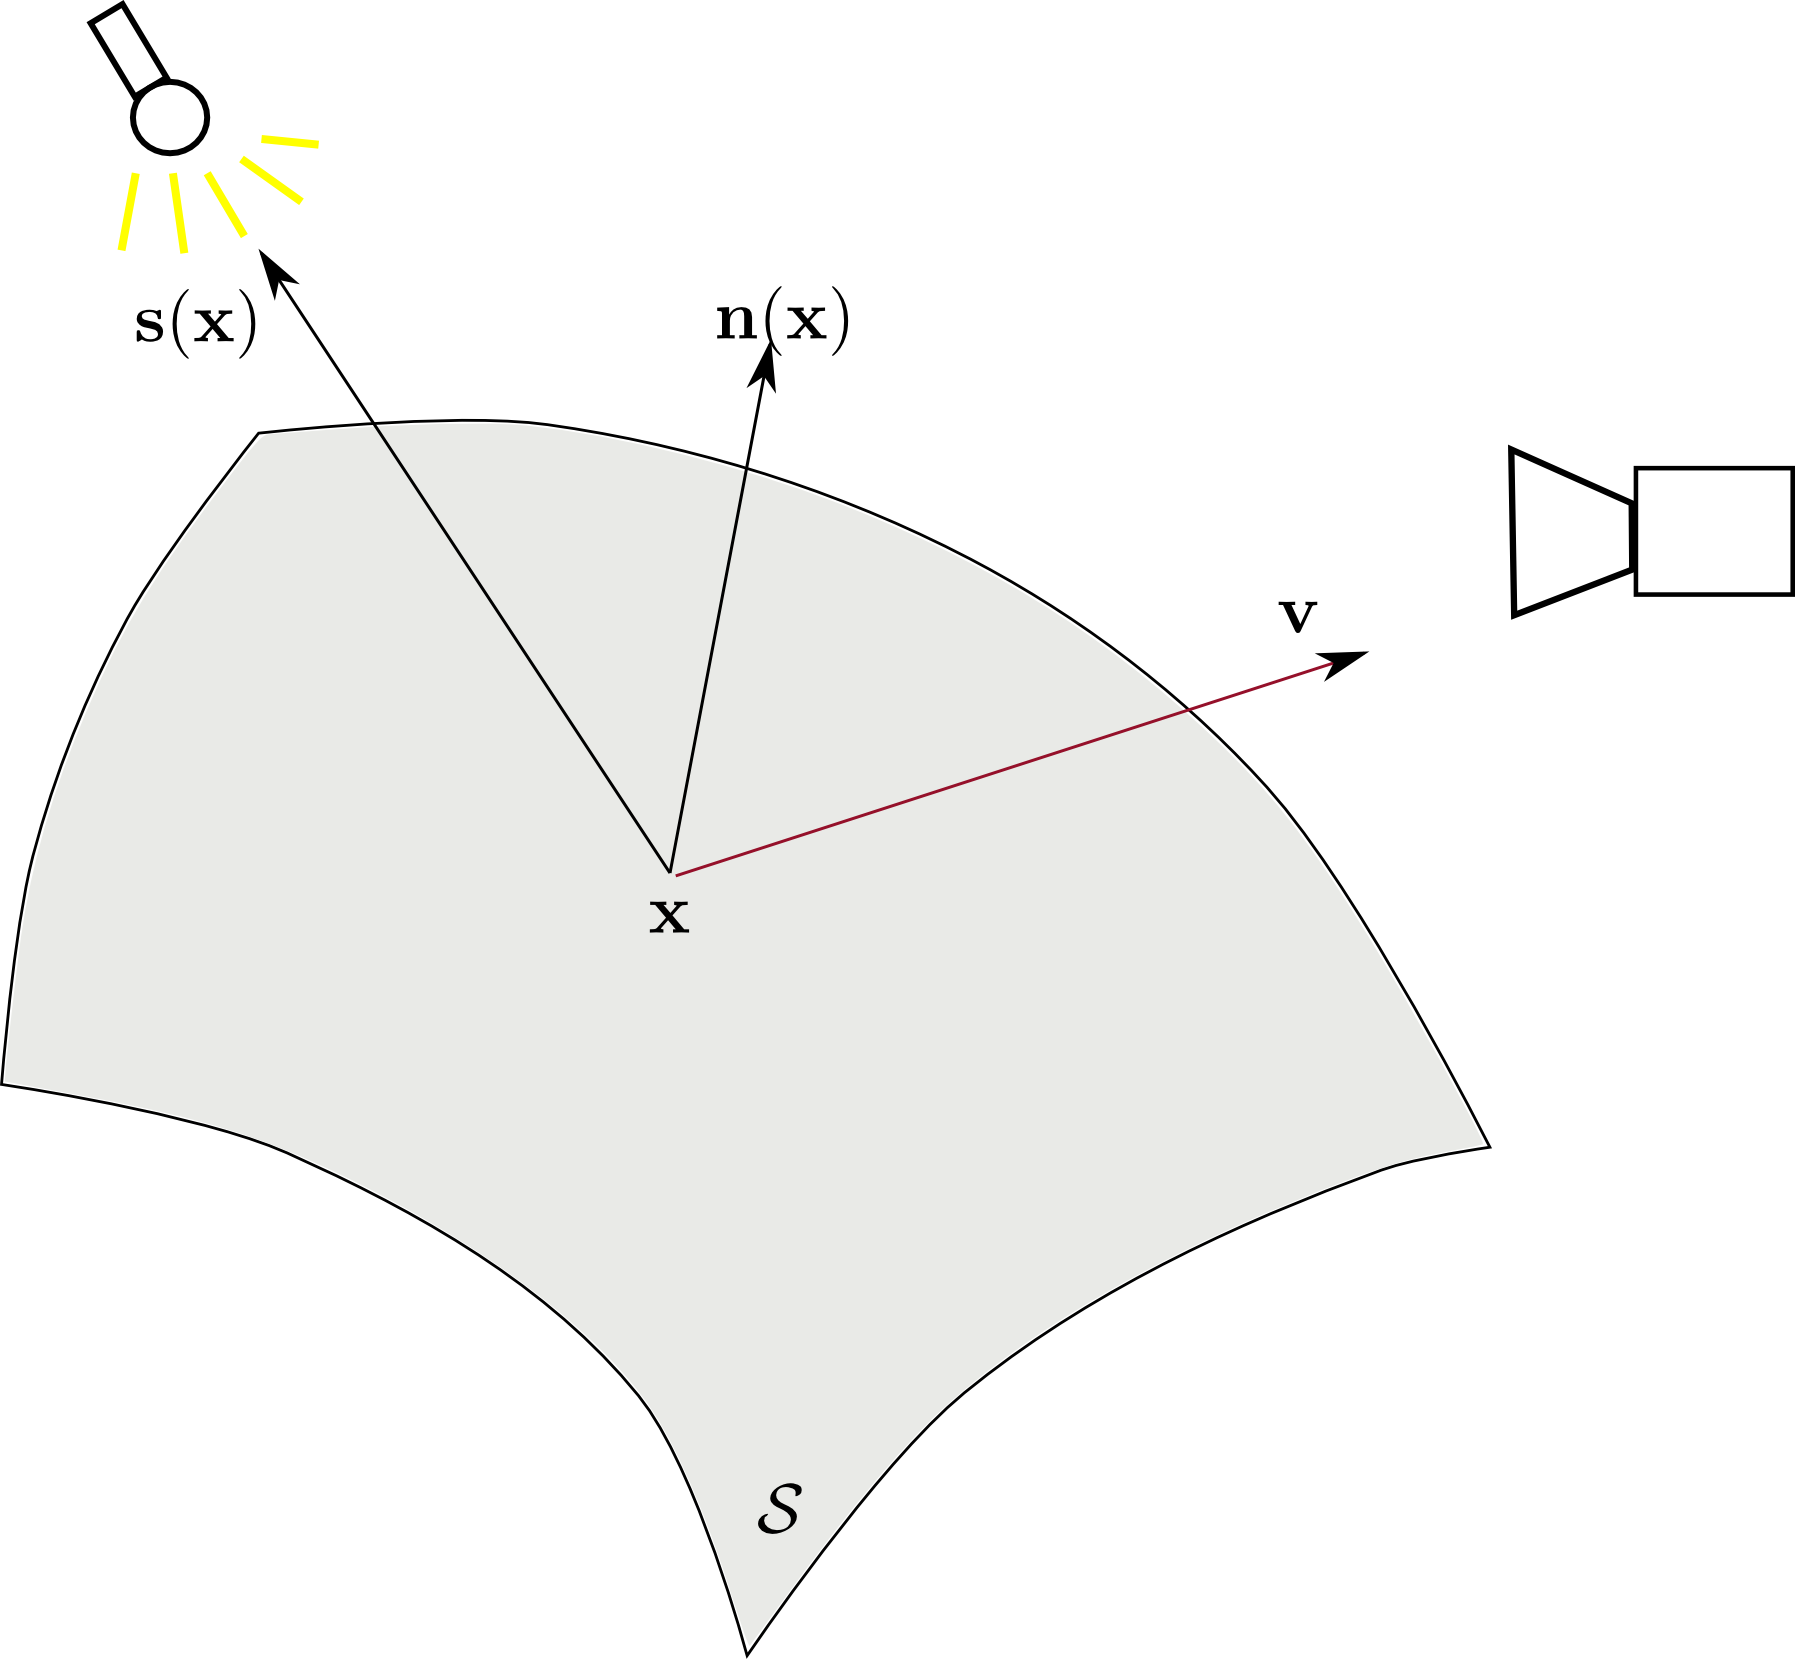
\includegraphics[width=0.456\textwidth]{FIGURES/reflectance}}
    \only<2->{
\includegraphics[width=0.456\textwidth]{FIGURES/reflectance2}}
  \end{center}
  \pause
  \begin{itemize}
  \item Luminance emitted by punctual object $\bx$ on a surface $\Ss$
    with normal direction $\bn(\bx)$ at $\bx$, in emission direction $\bv$
    characterized by spherical angles $(\theta_e,\phi_e)$ w.r.t $\bn(\bx)$:
    $$
    L(\bx,\theta_e,\phi_e)
    =\int_{\theta_i=0}^{\frac\pi2}\int_{\phi_i=0}^{2\pi}\kappa(\bx,\theta_i,\phi_i,\theta_e,\phi_e)
    \bar{L}(\theta_i,\phi_i)\sin\theta_i\,d\theta_id\phi.
    $$
    \pause
  \item Complicated equation, used in Computer Graphics. In Vision, try to guess a
    workable form for the reflection.
  \end{itemize}
\end{frame}



\begin{frame}{Specular Vs. Matte Objects} 
  \begin{center}
    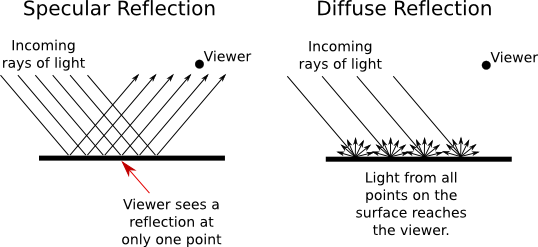
\includegraphics[width=0.6\textwidth]{FIGURES/specular_diffuse_reflection}
  \end{center}
  The two most standard reflection models: specular: mirror like surface, diffuse: rough
  surface (at very small scale): Lambertian model.  Others, very polular: Phong, Gouraud,
  Torrance-Sparrow etc\dots especially useful in Computer Graphics.
\end{frame}


\begin{frame}[t]{Diffuse Reflection}
  \begin{center}
    \begin{columns}
      \begin{column}{0.5\textwidth}
        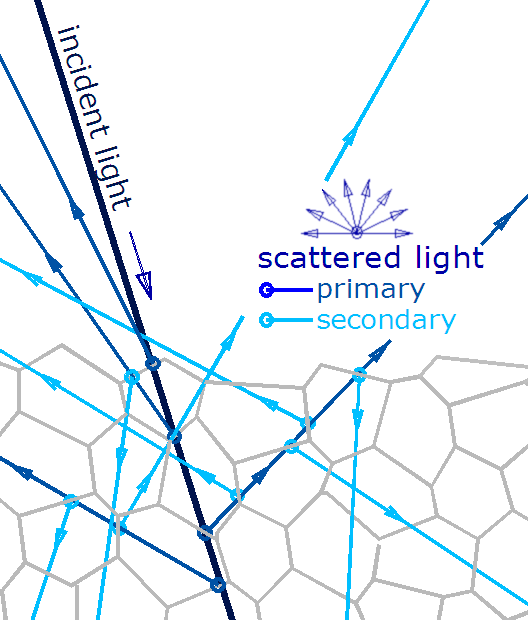
\includegraphics[width=0.95\textwidth]{FIGURES/Diffuse_reflectionGIANNI46WIKI}
      \end{column}
      \begin{column}{0.5\textwidth}
        \onslide<2->
        {
          Rough surface at micro-scale.\\~\\
          \begin{itemize}
          \item Light bounces.
          \item Reflections in all directions
          \item Some light is absorbed.
          \item Only a percentage of light energy is reemitted.
          \end{itemize}
        }
      \end{column}
    \end{columns}
  \end{center}
  \vfill
 {\fontsize{6}{6}\selectfont Image Source GianniG46, Wikipedia}
\end{frame}



\begin{frame}
\frametitle{Lambert's Cosine Law}
\begin{block}{Reflectance}
\begin{itemize}
  \item Linearised Lambertian model: $I(\mathbf{p}) = \rho(\mathbf{x}) \mathbf{s}(\mathbf{x}) \cdot \mathbf{n}(\mathbf{x})$
  \item $\rho({\bf x})$ is the \emph{albedo} at ${\bf x}$ -- material light absorption property, $\rho\in [0,1]$.
  Assumes matte material such as chalk... 
\end{itemize}
\end{block}
\begin{columns}
 \begin{column}{0.45\textwidth}
 \begin{center} 
 \uncover<2->{\includegraphics[width=0.9\textwidth]{FIGURES/lambertslaw1}}
 \end{center}
 \end{column}
 \begin{column}{0.51\textwidth}
 \begin{center}
 \uncover<3->{\includegraphics[width=0.9\textwidth]{FIGURES/lambertslaw2}}
 \end{center}
 \end{column}
 \end{columns}
 \uncover<4->{ 
   \begin{block} {In words}
     \begin{itemize}
     %\item Only a percentage of received light is reflected, the rest is absorbed by material: albedo.
     \item Local orientation of object w.r.t. light: In surface 1:
       surface area matches ray ``section''. In surface 2: surface
       area larger than ray section, but receive same amount of light.
     \end{itemize}
   \end{block}
 }
\end{frame}


\begin{frame}[t]{Shadows}
  \begin{center}
    \includegraphics[width=0.7\textwidth]{FIGURES/selfcast_shadows}
  \end{center}
  \begin{itemize}
  \item Self shadow: surface is behind the light source. $\bs\cdot\bn \leq 0$.
  \item Cast shadow: part of the scene occludes another part.
  \end{itemize}
\end{frame}

\begin{frame}[t]{Shadows again}
  \begin{center}
    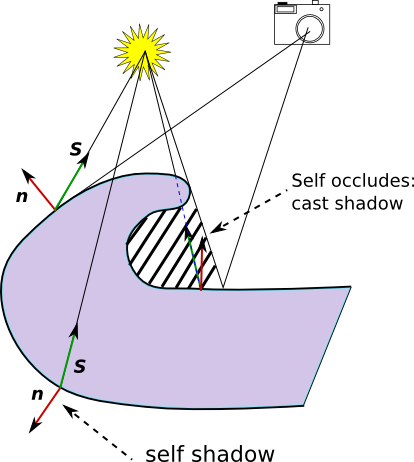
\includegraphics[width=0.5\textwidth]{FIGURES/shadows}
  \end{center}  
  \begin{itemize}
  \item Lambert's law and self-shadows: $I = \rho\max(\bs\cdot\bn,0)$.
  \item Cast shadows: Non local phenomenon, Lambert's law is local...
  \end{itemize}
\end{frame}


\section{Photometric Stereo}

\begin{frame}[t]{Type of Light Sources}
  \begin{center}
    \includegraphics[width=0.6\textwidth]{FIGURES/farlight}
  \end{center}
  \begin{itemize}
  \item Top: near light source, radial.
  \item Bottom: far light source: parallel. \myemph{Our choice in these lectures}.
  \item Other types?
  \end{itemize}
\end{frame}

\begin{frame}[t]{Shape From Shading (SfS) -- B. Horn 1970 }
  \begin{center}
    
\includegraphics[width=0.456\textwidth]{FIGURES/reflectance2}
  \end{center}
  \begin{itemize}
  \item Use Lambert's Law to gain information on visible surface via normal vector $\bn(\bx)$. 
  \item Need link between surface equations and normal vector.
  \end{itemize}  
\end{frame}


\begin{frame}[t]{Settings}
  \begin{itemize}
  \item Representation of the surface. Assume surface parameterized by $(u,v)\mapsto \Ss(u,v)\in \RR^3$. Even better: \myemph{depth map}:
    $$
    S(u,v) = [u,v,z(u,v)]^T:\text{ Monge Patch}.
    $$
  \end{itemize}
  \pause
  \begin{columns}
    \begin{column}{0.38\textwidth}
      \begin{center}
        \uncover<2->{\includegraphics[width=1.0\textwidth]{FIGURES/surfacediffgeom}}
      \end{center}      
    \end{column}
    \begin{column}{0.62\textwidth}
      Tangent vectors at $\bx(u,v) = [u,v,z(u,v)]^\top$
      $$
      \pder{\Ss}{u}=S_u=
      \begin{bmatrix}
        1\\ 0\\ \pder{z}{u}
      \end{bmatrix},\quad
      \pder{\Ss}{v}=\Ss_v
      \begin{bmatrix}
        0\\ 1\\\pder{z}{v}
      \end{bmatrix},\quad
      $$      
    \end{column}
  \end{columns}
\pause
  \begin{itemize}
  \item Normal vector $\bn(u,v) = \bn(\bx(u,v))$
    $$
    \bn(\bx) = \frac{\Ss_u\times\Ss_v}{|\Ss_u\times\Ss_v|} = \frac{1}{\sqrt{|\nabla z|^2 + 1}}
      \begin{bmatrix}
        -z_u\\-z_v\\1
      \end{bmatrix}
    $$
  \end{itemize}
\end{frame}


\begin{frame}[t]{Camera Model, Lambertian SfS equations }
  \begin{itemize}
  \item Two Choices: pinhole and orthographic.
  \item \color{blue}{Orthographic Camera Model}.
    \begin{itemize}
    \item $[x=u,y=v,z]\mapsto [u,v]$: orthographic projection.
    \item Formula from previous slide: Coordinates of normal vector in orthographic projection:
      $$
      \bn_z = \frac{1}{\sqrt{|\nabla z|^2 + 1}}[-z_u, -z_v, 1]^T
      $$
    \end{itemize}
  \item \color{blue}{Pinhole Camera model}.
    \begin{itemize}
    \item Projection
      $$  
      \begin{bmatrix}
        x\\y\\z
      \end{bmatrix}\mapsto
      \begin{bmatrix}
        u=\frac{fx}{z}\\v=\frac{fy}{z}
      \end{bmatrix}
      $$
    \item Normal vector in camera coordinates: complicated!
      $$
      \bn_z = \frac{1}{\sqrt{|\nabla z|^2 + \left(\frac{z + [u,v]\nabla z}{f}\right)^2}}
      \left[-z_u, -z_v, \frac{z + [u,v]\nabla z}{f}\right]^T
      $$ 
    \end{itemize}
  \end{itemize}\pause
  \begin{center}
    \large \color{blue}{Solve for $z$: $I = \rho \bn_z\cdot\bs$}\\
    \huge \color{red}{Complicated Math and Research Topics}
  \end{center}
\end{frame}

\begin{frame}[t]{Examples, Problems}
  \begin{center}
    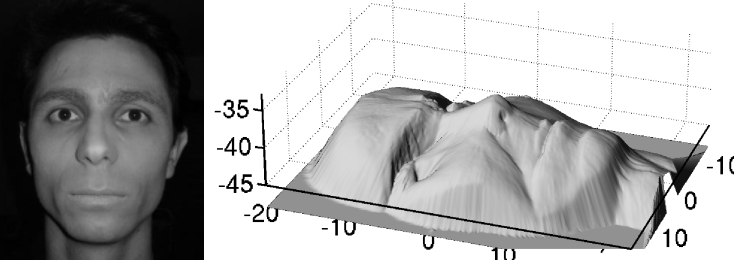
\includegraphics[width=0.7\textwidth]{FIGURES/pradosFaceAndReconstructionPG}
  \end{center}
  \pause
  \begin{center}
    \onslide<2->{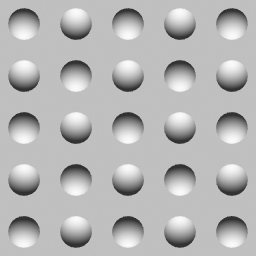
\includegraphics[width=0.35\textwidth]{FIGURES/shading02}}
  \end{center}
\end{frame}


\begin{frame}[t]{SfS (Counter)Example}
  \begin{center}
    \begin{tabular}[h]{cc}
      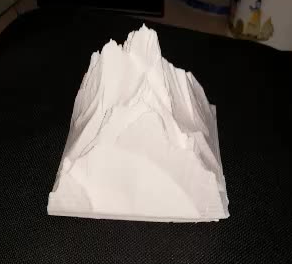
\includegraphics[width=0.34\textwidth]{IMAGES/Lena1SfS}~~~~~~&
      \onslide<2->{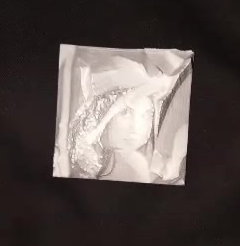
\includegraphics[width=0.30\textwidth]{IMAGES/Lena2SfS}}
    \end{tabular}~\\
    \onslide<3->{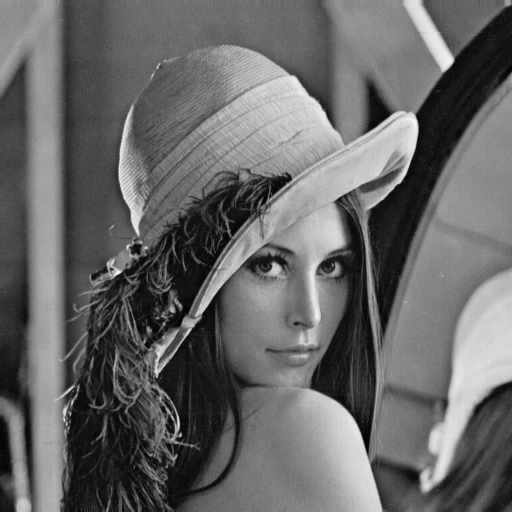
\includegraphics[width=0.30\textwidth]{IMAGES/lena}}
  \end{center}
\end{frame}

\begin{frame}[t]{Why Does It Go Wrong}
  Assume Light $\bs$ known and constant (far light source with known intensity).\color{red}{Per Pixel:}
  \begin{itemize}
  \item Number of unknowns: 
    \begin{itemize}
    \item Normal vector $\bn(u,v)$, 3 components $[\bn_1,\bn_2,\bn_3]$, but 
      $$\|\bn\|=1: \bn_1^2 + \bn_2^2 + \bn_3^2 = 1.$$
      2 degrees of freedom (DoF).
    \item Albedo $\rho(u,v)$: 1 value, 1 DoF.
    \item Total: 3 DoF.
    \end{itemize}\vfill
    \item Known information per pixel:
      \begin{itemize}
      \item Reflectance $I(u,v) = \rho(u,v) \bs\cdot \bn(u,v)$: 1 equation linking 3 unknowns.
      \end{itemize}\vfill
    \item Remaining DoFs: 2.
    \item For unambiguous solution, need remaining DoF = 0.
    \item In counterexample, 1DoF removed by assuming $\rho(u,v) \equiv 1$: \myemph{Wrong!}
  \end{itemize}

\end{frame}



\begin{frame}[t]{Woodham Original PS -- 1980}
  \vfill
  \begin{itemize}[<+->]
  \item How to remove Degrees of Freedom?\vfill
  \item Woodham Solution: Use more images $I^1$, $I^2$,\dots, $I^k$. \vfill
  \item Don't change Camera Position -- keep same depth function, normals, change lights.\vfill
  \item $k$ far (parallel) light sources $\bs^1$,\dots,$\bs^k$: $k$ equations
    $$
    \begin{cases}
      I^1(u,v) &= \rho(u,v)\bs^1\cdot\bn(u,v)\\
      I^2(u,v) &= \rho(u,v)\bs^2\cdot\bn(u,v)\\
      \hdots & \hdots\\
      I^k(u,v) &= \rho(u,v)\bs^k\cdot\bn(u,v)\\
    \end{cases}
    $$
    $$
    (\bs^i\cdot \bn = \bs_1^i\, \bn^1 + \bs_2^i\,\bn_2 + \bs_3^i\, \bn_3)
    $$
    \vfill
  \item Which $k$ to choose? 3 DoF: $k\geq 3$. Exactly 3, more?\vfill
  \item Answer is \myemph{geometric}!
  \item From $(u,v)\mapsto \bn(u,v)$ to surface? Integration of normals: \color{red}{out of scope; Matlab / Python functions will be provided.}
  \end{itemize}
\end{frame}


\begin{frame}[t]{Linear System for Normal + Albedo}
  \begin{itemize}[<+->]
  \item Woodham idea: Normal + Albedo Simultaneously
    $$
    \bm := \rho\bn,\quad \rho = \|\bm\|, \bn = \frac{\bm}{\|\bm\|}
    $$
  \item
    Problem if $\rho = 0$: absolutely black object -- shadow.
  \item $k$ Lambert's laws \myemph{for a given pixel} at $[u,v]$
    $$
    \udesc{\text{Image vector } \bI, k\times 1}{\begin{bmatrix}
        I_1\\
        I_2\\
        \vdots\\
        I_k
      \end{bmatrix}
    }
    =
    \udesc{\text{Light matrix }M_\bs, k\times 3}{\begin{bmatrix}
        \bs_1^1 & \bs_1^2 & \bs_1^3\\
        \bs_2^1 & \bs_2^2 & \bs_2^3\\
        \vdots & \vdots & \vdots \\
        \bs_k^1 & \bs_k^2 & \bs_k^3\\
      \end{bmatrix}}
    \begin{bmatrix}
      \bm_1\\\bm_2\\\bm_3
    \end{bmatrix}
    $$
  \item Number of solutions?
  \item Can vary from none to a lot!
  \end{itemize}
\end{frame}




\begin{frame}{Linear Algebra Again}
  \begin{itemize}
  \item System of equations in 2 unknown.
  \end{itemize}
  \begin{center}
    \includegraphics[width=0.8\textwidth]{FIGURES/sols2unknowns}
  \end{center}
  \begin{itemize}
  \item Need at least 2 \myemph{independent} equations! ...but not 3!
  \item For 3 or more: concept of ``closest solution in least squares''. 
  \end{itemize}
\end{frame}

\begin{frame}[t]{In 3D}
  \begin{center}
    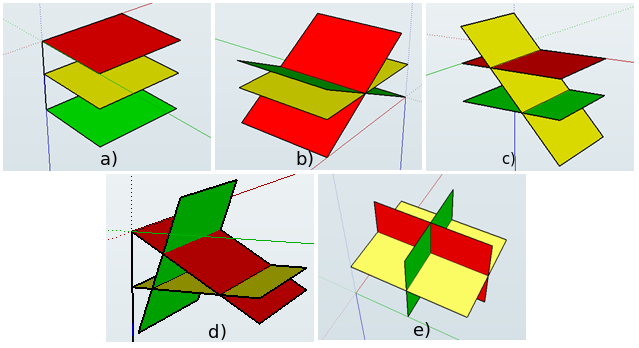
\includegraphics[width=0.8\textwidth]{FIGURES/interplanes} ~\\
  \end{center}
  {\small Same light source, incompatible measurements, b) coplanar
    light sources, compatible measurements, c) 2 light source, 3
    incompatible measurements, d) coplanar light sources, incompatible
    measurements, e) 3 non coplanar light sources  
  }  \vfill
  {\fontsize{6}{6}\selectfont Picture from Guillermo Bautista,
    mathandmultimedia.com}
\end{frame}



\begin{frame}[t]{What Can Go Wrong?}
  \begin{itemize}
  \item Parameters / devices:
    \begin{itemize}
      \item Measurement errors: Camera?
      \item Coplanar light sources: example?
      \end{itemize}
    \item Reflectance
      \begin{itemize}
      \item Lambert's law only valid for matte materials: specularities.
      \item Shadows / penumbra: non black cast shadow areas.
      \end{itemize}
    \item More?
  \end{itemize}
  \begin{center}
    \onslide<2->{\includegraphics[width=0.36\textwidth]{FIGURES/camresp}}~~~~~
    \onslide<3->{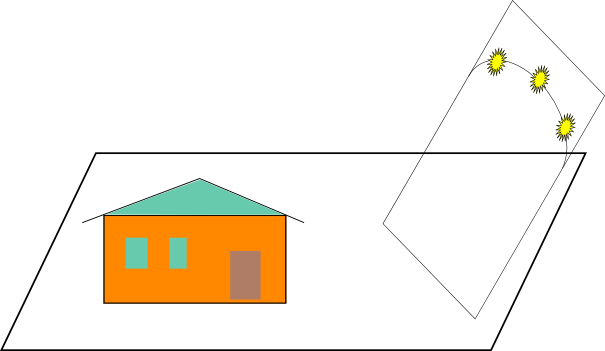
\includegraphics[width=0.4\textwidth]{FIGURES/coplanarsun}}\\
    \onslide<4->{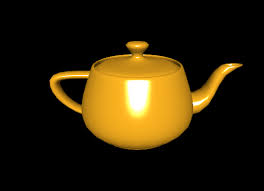
\includegraphics[width=0.3\textwidth]{FIGURES/teapotspec}}~~~~
    \onslide<5->{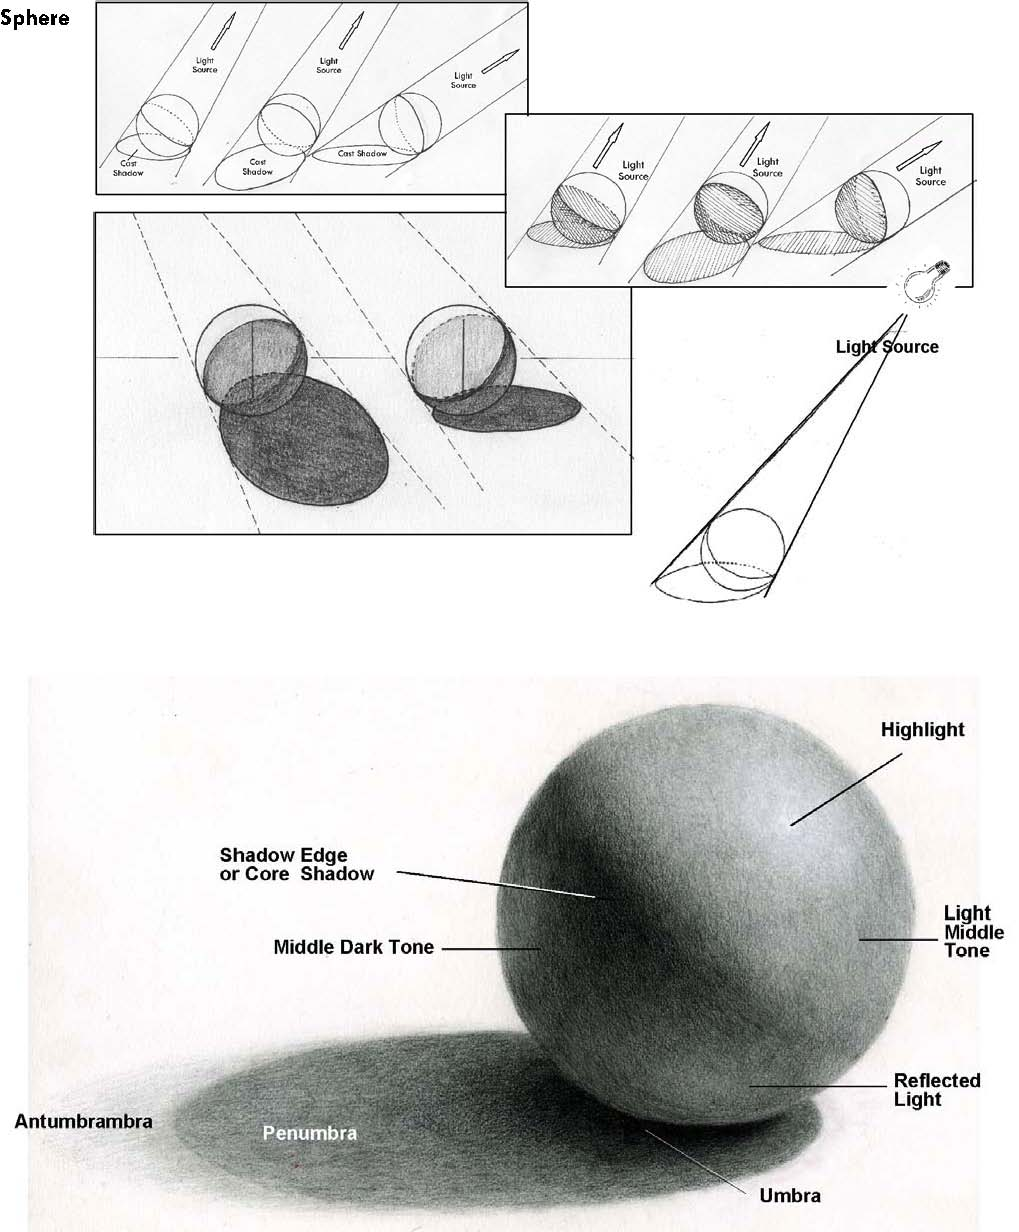
\includegraphics[width=0.35\textwidth]{FIGURES/penumbra}}
  \end{center}
\end{frame}


\begin{frame}[t]{Solving For Normals: Pseudo-Inverse Approach}
  Assume 3 or more non coplanar light sources.\\\vfill
  \begin{itemize}
  \item Equation $\bI = M_\bs\,\bm$ may not have solution if $\bM_\bs$ is $k\times 3$, $k> 3$.
  \item Via Moore-Penrose Pseudo-Inverse $M_\bs^\dagger$, solution of 
    $$
    \bm \text{ such that } \|\bI - M_\bs \bm\|^2 = \min:\quad \bm = M_\bs^\dagger\bI.
    $$
  \end{itemize}
  \flushleft{\myemph{Pros}}.
  \begin{itemize}
  \item Good news: Matlab \texttt{pinv} function, Python \texttt{pinv}
    function in package \texttt{numpy.linalg}.
  \end{itemize}
  \flushleft{\myemph{Cons}}.
  \begin{itemize}
  \item Does not separate wrong and accurate measurements.
  \end{itemize}
\end{frame}



\begin{frame}[t]{Solving For Normals: Equations Selection - I}
  \flushleft{\myemph{In a nutshell}}.~\\
  \begin{itemize}
  \item Per pixel: find best constraints: 3 ``good measurements''
    $I^{a}$, $I^{b}$, $I^{c}$ and corresponding ``good lights''
    $\bs^{a}$, $\bs^{b}$, $\bs^{c}$.
    $$
    \udesc{\bI_{abc}}{
      \begin{bmatrix}
        I^{a}\\I^{b}\\I^{c}
      \end{bmatrix}
    }
    = 
    \udesc{M_{abc}}
    {
      \begin{bmatrix}
        \bs_1^{a} & \bs_2^{a} & \bs_3^{a}\\
        \bs_1^{b} & \bs_2^{b} & \bs_3^{b}\\
        \bs_1^{c} & \bs_2^{c} & \bs_3^{c}\\
      \end{bmatrix}
    }
    \begin{bmatrix}
      \bm^1\\\bm^2\\\bm^3
    \end{bmatrix}
    $$
  \end{itemize}
  \flushleft{\myemph{Good measurements}}.~\\
  \begin{itemize}
  \item $I_{i}$ good measurement: not too small (shadow, penumbra) and not too large (saturation, potential specularity).
  \item Good light sources: $\det{M_{abc}}$ as large as possible.
  \end{itemize}
\end{frame}

\begin{frame}[t]{Solving For Normals: Equations Selection - II}
  \flushleft{\myemph{Pros}}.~\\
  \begin{itemize}
  \item Best system of equations per pixel.
  \end{itemize}
  \vfill
  \flushleft{\myemph{Cons}}.~\\
  \begin{itemize}
  \item Lack of spatial coherence: different lights can be chosen for neighbor pixels.
  \item Need thresholds for intensities: parameters of the algorithm.
  \item More complicated to code.
  \end{itemize}\vfill 
  \flushleft{\myemph{Size Matters}}.~\\
  \begin{itemize}
  \item For relatively small $k$: equation selection can be a good idea.
  \item For very large $k$ (1000, more...) pseudo-inverse very good: statistical reason.
  \end{itemize}
  
\end{frame}


\begin{frame}[t]{Algorithm in a Nutshell}
  \vfill
  \flushleft{\myemph{Input}}.~\\
  \begin{itemize}
  \item $k$ known parallel light sources $\bs_1,\dots \bs_k$. $k$
    recorded images $I_1,\dots,I_k$.
  \end{itemize}
  \vfill
  \flushleft{\myemph{Normals and Albedo recovery}}.~\\
  \begin{itemize}
  \item For each (valid) pixel $[u,v]$ in image domain:\vfill
    \begin{enumerate}
    \item Solve $\bm(u,v)$ either via pseudo-inverse or equation selection.\vfill
    \item Get albedo and normal:
      $$
      \rho(u,v) = \|\bm(u,v)\|,\quad \bn(u,v) = \frac{1}{\rho(u,v)}\bm(u,v).
      $$
    \end{enumerate}
    \vfill
  \end{itemize}
  \flushleft{\myemph{Surface Recovery}}.~\\
  \begin{itemize}
  \item Get surface from normals via surface integration.
  \item May ``paint surface'' with albedo.
  \end{itemize}
  \vfill
  
\end{frame}



\begin{frame}{Robust Statistics}
  \begin{itemize}
  \item Classical Least-Square estimate may fail due to outliers in data
  \end{itemize}
  \begin{center}
    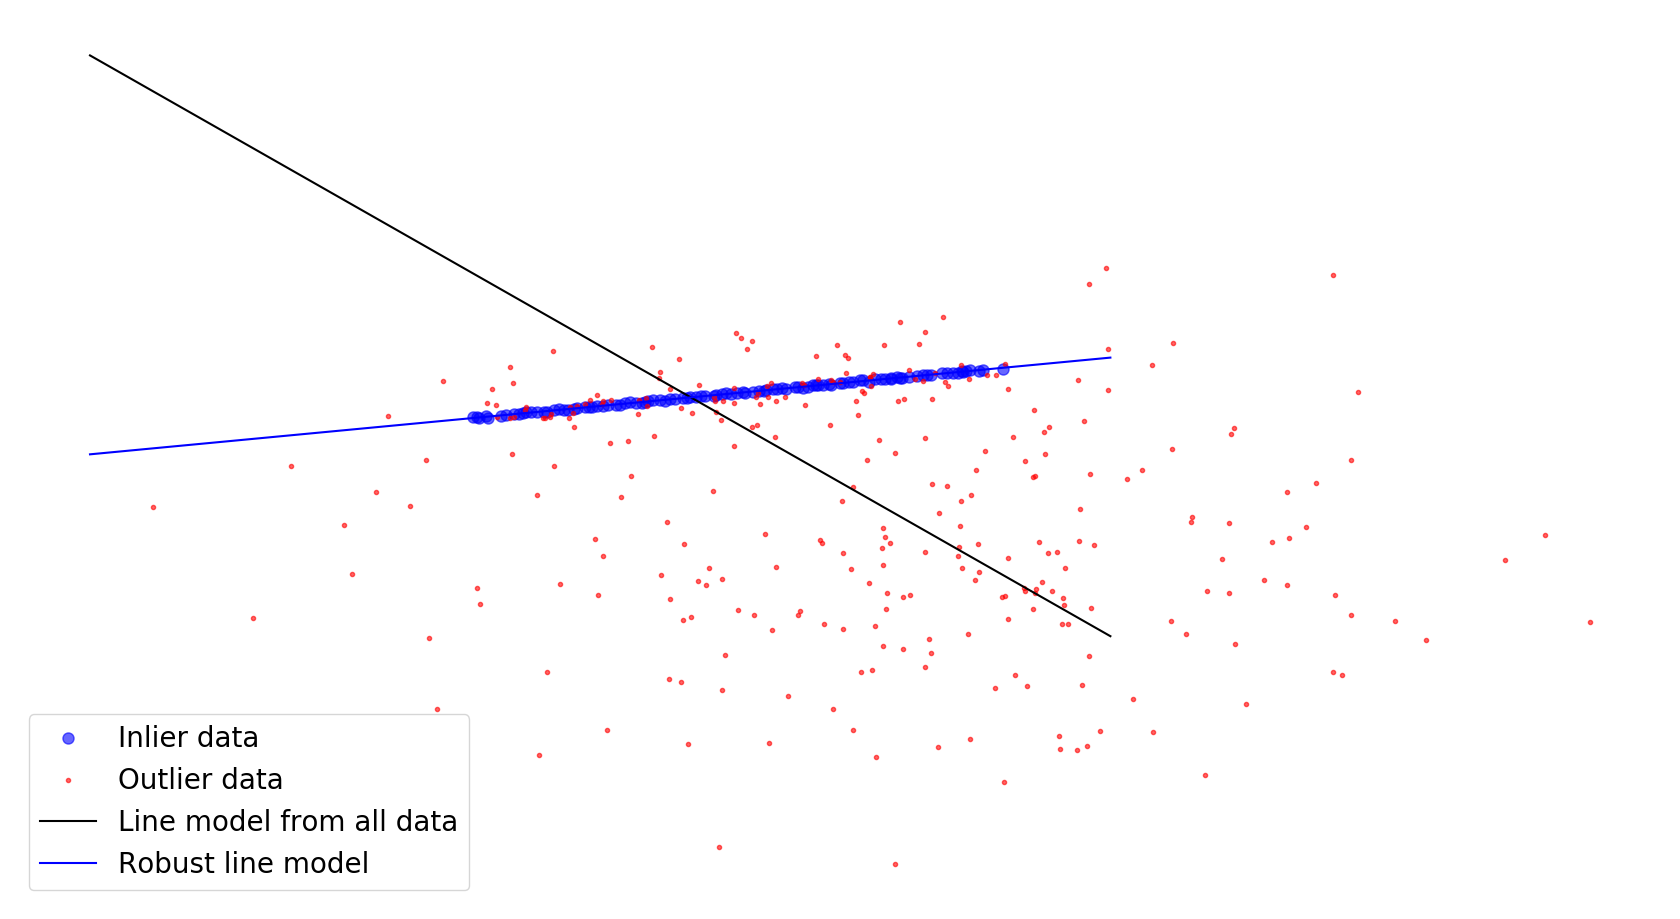
\includegraphics[width=0.8\textwidth]{FIGURES/robust_ransac_line}
  \end{center}
  \begin{itemize}
  \item LS estimated line: the black one.
  \item The correct line: blue.
  \item Extremely active research topic, mixing statistics and very complicated optimisation.
  \item We explore a classical one: RANSAC
  \end{itemize}
\end{frame}


\begin{frame}{A Classical in Computer Vision: RANSAC}
  \begin{itemize}
  \item RANSAC = RANdom SAmplic Consensus: Fishler \& Bolles, 1981.
  \item Idea: if the data contains enough \emph{inliers}, random sampling should provided
    some, after possibly many repetitions.
  \end{itemize}
  \vfill
  \begin{center}
      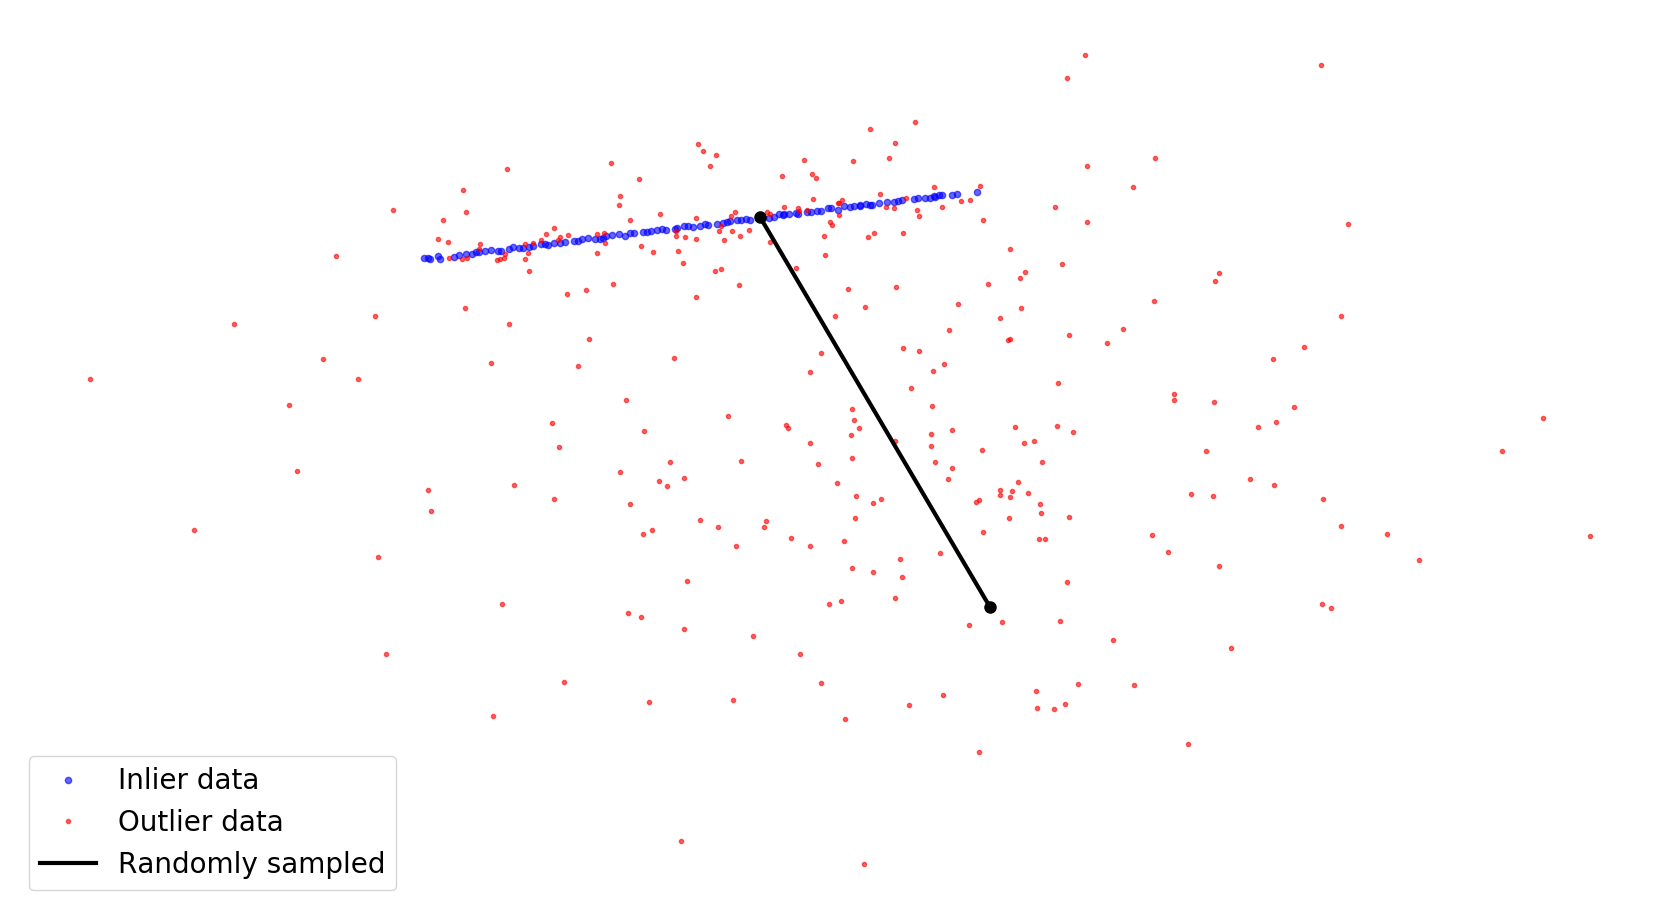
\includegraphics[width=0.8\textwidth]{FIGURES/ransac_random_sample_line0}
  \end{center}
\end{frame}

\begin{frame}{A Classical in Computer Vision: RANSAC}
  \begin{itemize}
  \item RANSAC = RANdom SAmplic Consensus: Fishler \& Bolles, 1981.
  \item Idea: if the data contains enough \emph{inliers}, random sampling should provided
    some, after possibly many repetitions.
  \end{itemize}
  \vfill
  \begin{center}
      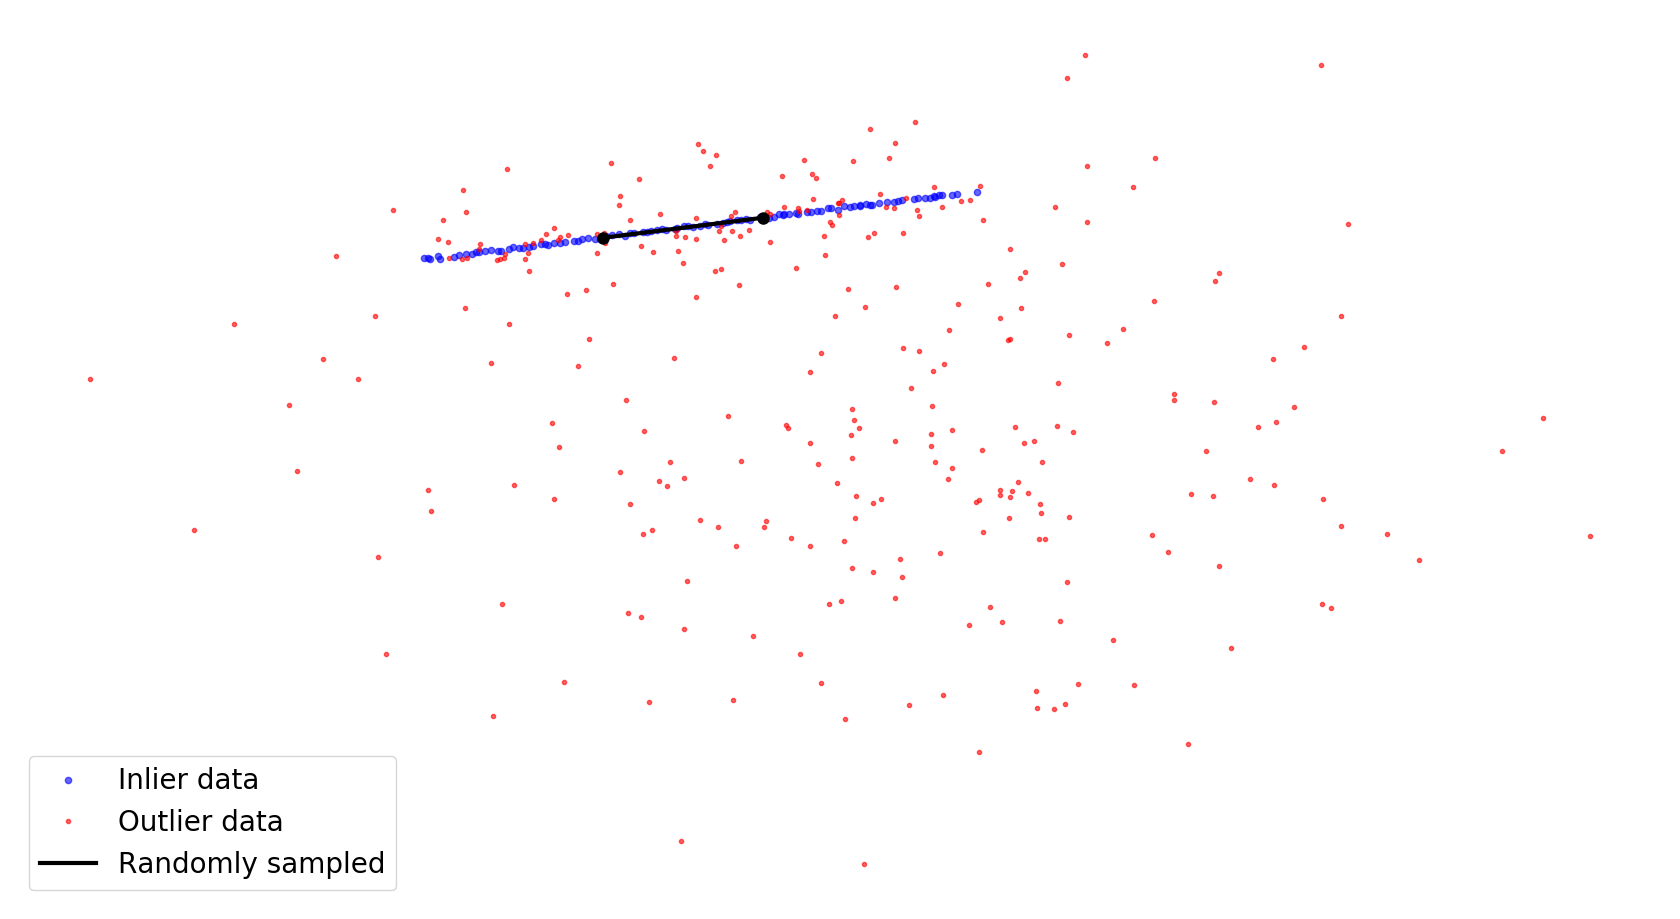
\includegraphics[width=0.8\textwidth]{FIGURES/ransac_random_sample_line1}
  \end{center}
\end{frame}

\begin{frame}{A Classical in Computer Vision: RANSAC}
  \begin{itemize}
  \item RANSAC = RANdom SAmplic Consensus: Fishler \& Bolles, 1981.
  \item Idea: if the data contains enough \emph{inliers}, random sampling should provided
    some, after possibly many repetitions.
  \end{itemize}
  \vfill
  \begin{center}
      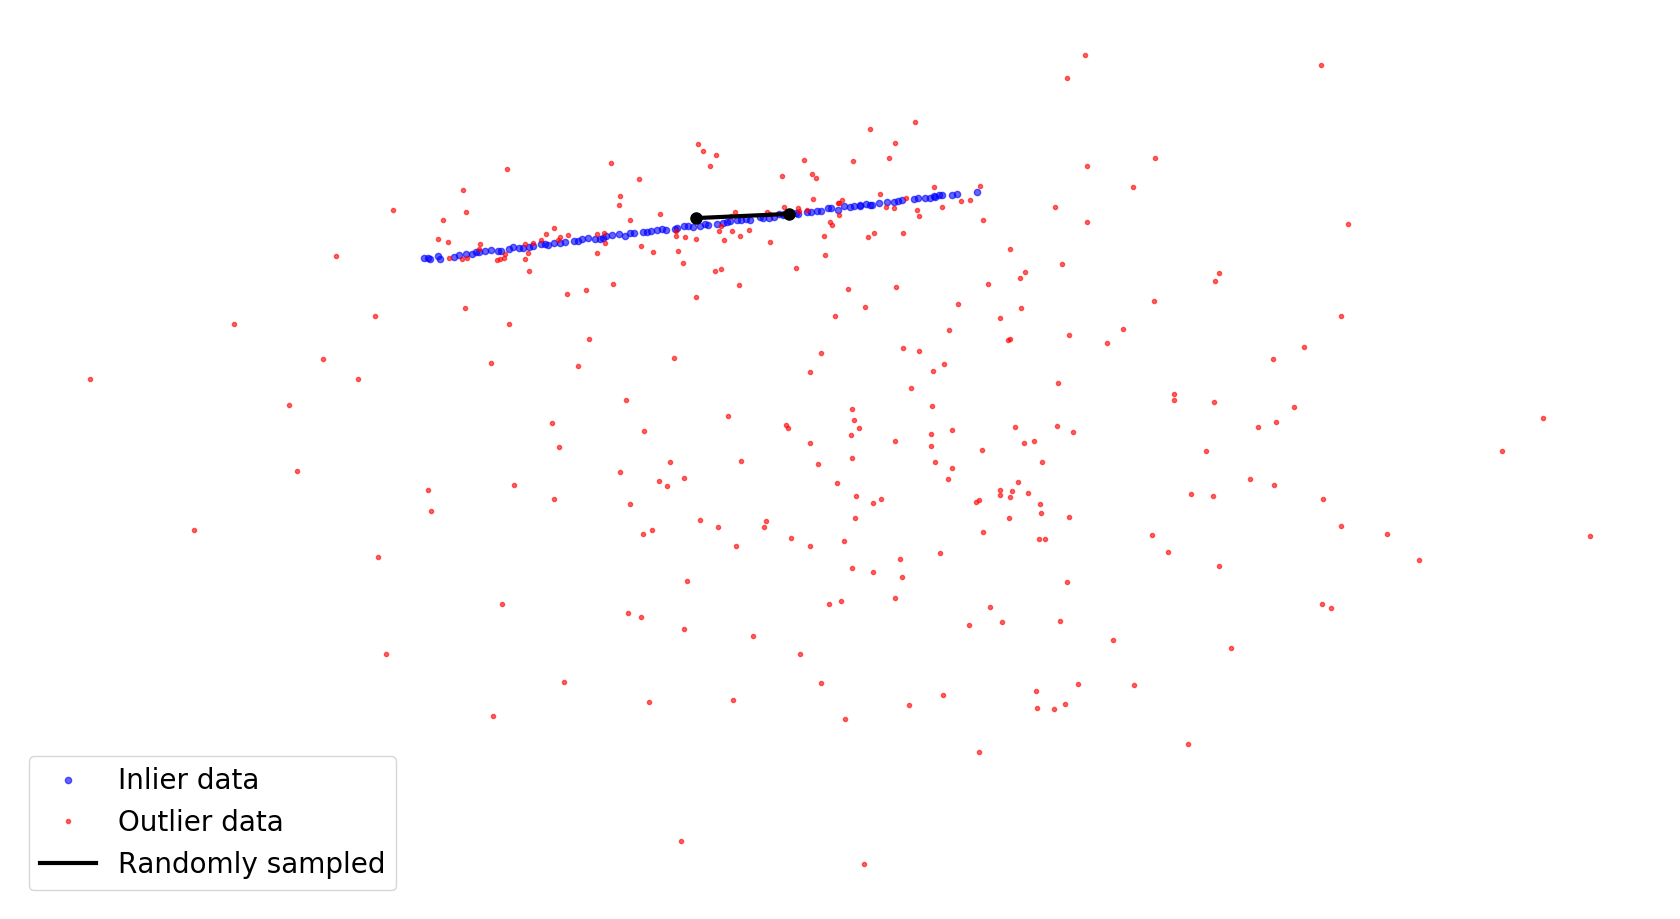
\includegraphics[width=0.8\textwidth]{FIGURES/ransac_random_sample_line2}
  \end{center}
\end{frame}



\begin{frame}{2D Line Fitting RANSAC}
  \begin{itemize}
  \item From two points $(x_1,y_1)$ and $(x_2, y_2)$: a line $L: y = ax + b$,
    $$
    y = \udesc{a}{\frac{y_2-y_1}{x_2-x_1}}x + \udesc{b}{\frac{y_1x_2-y_2x_1}{x_2-x_1}}
    $$
  \item Does it fit the data well enough?
  \item For each data point $(x_i, y_i)$: compute residual / fitting square error
    $$
    r_i = |y_i - ax_i - b|^2
    $$
  \item if $r_i < \tau$: predefined threshold: \myemph{declare $(x_i,y_i)$ inlier}.
  \item if $r_i \geq \tau$: \myemph{declare $(x_i,y_i)$ outlier}.
  \item Choose the \myemph{model} $(a,b)$ with \myemph{most} inliers.
  \item Reestimate the model \myemph{only from inliers} (least-squares)
  \end{itemize}
\end{frame}





\begin{frame}{Sample run in 2D: Bad}
  \begin{center}
      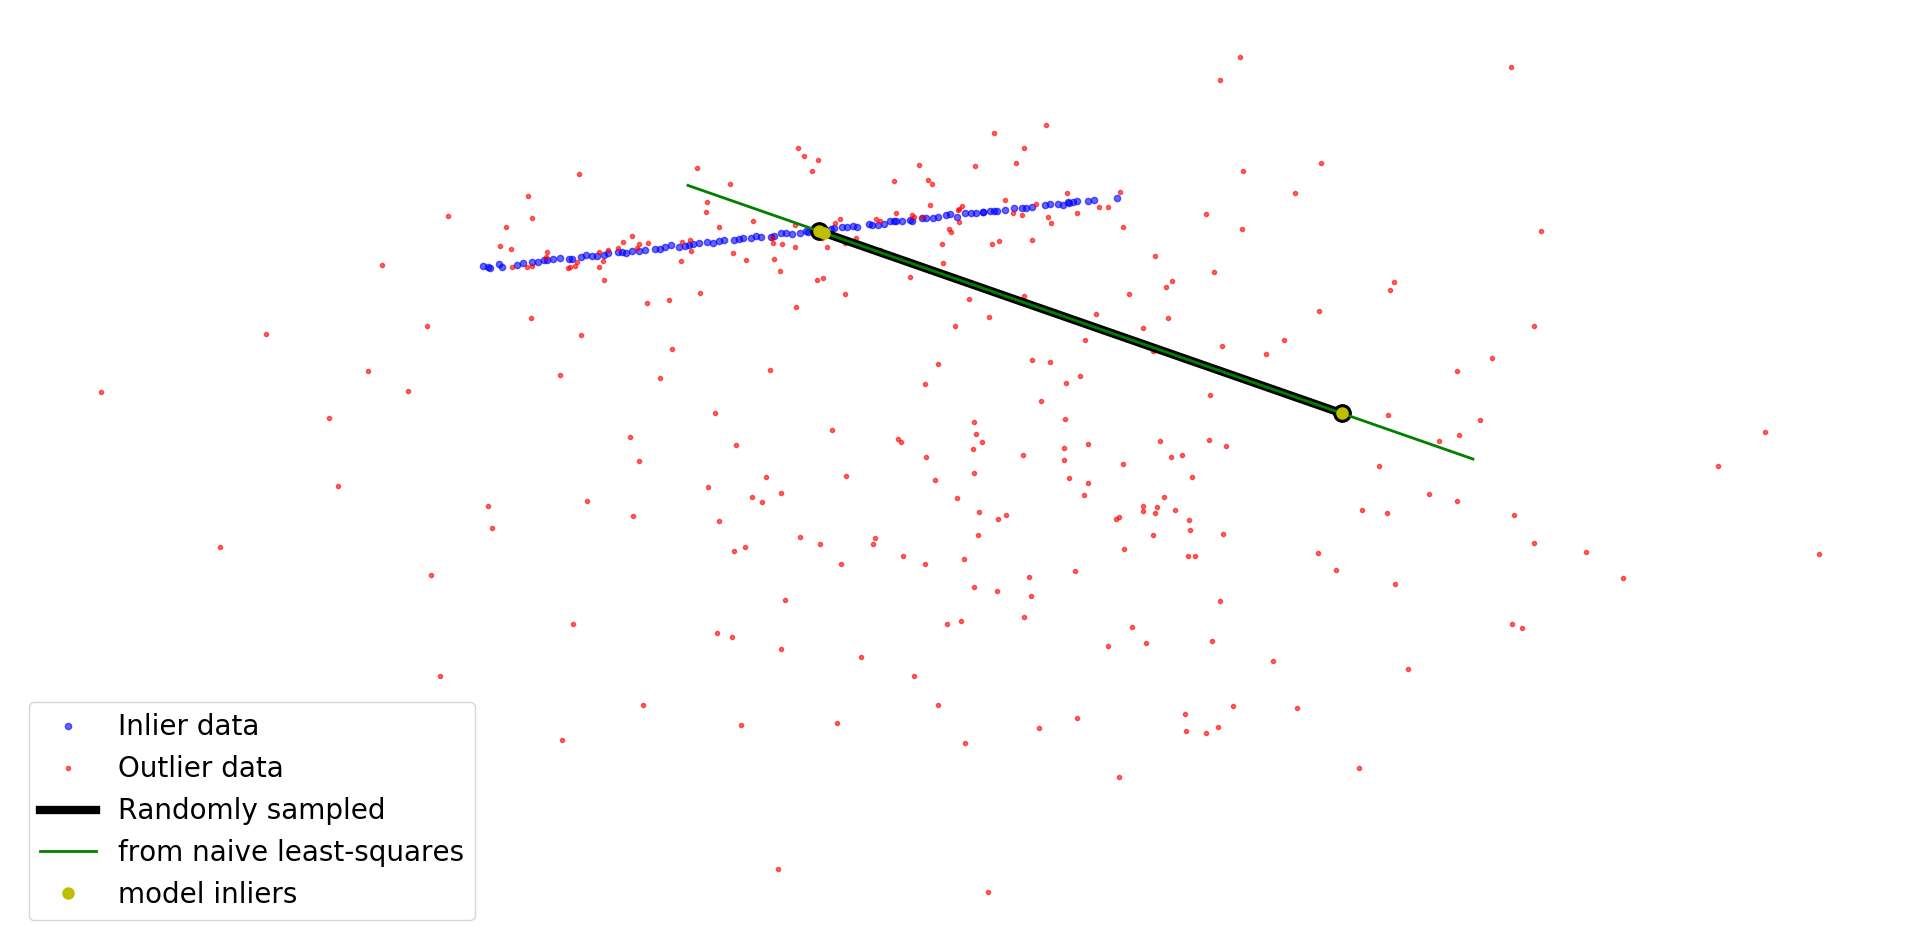
\includegraphics[width=0.95\textwidth]{FIGURES/ransac_trial_bad}
  \end{center}
\end{frame}


\begin{frame}{Sample run in 2D: Better}
  \begin{center}
      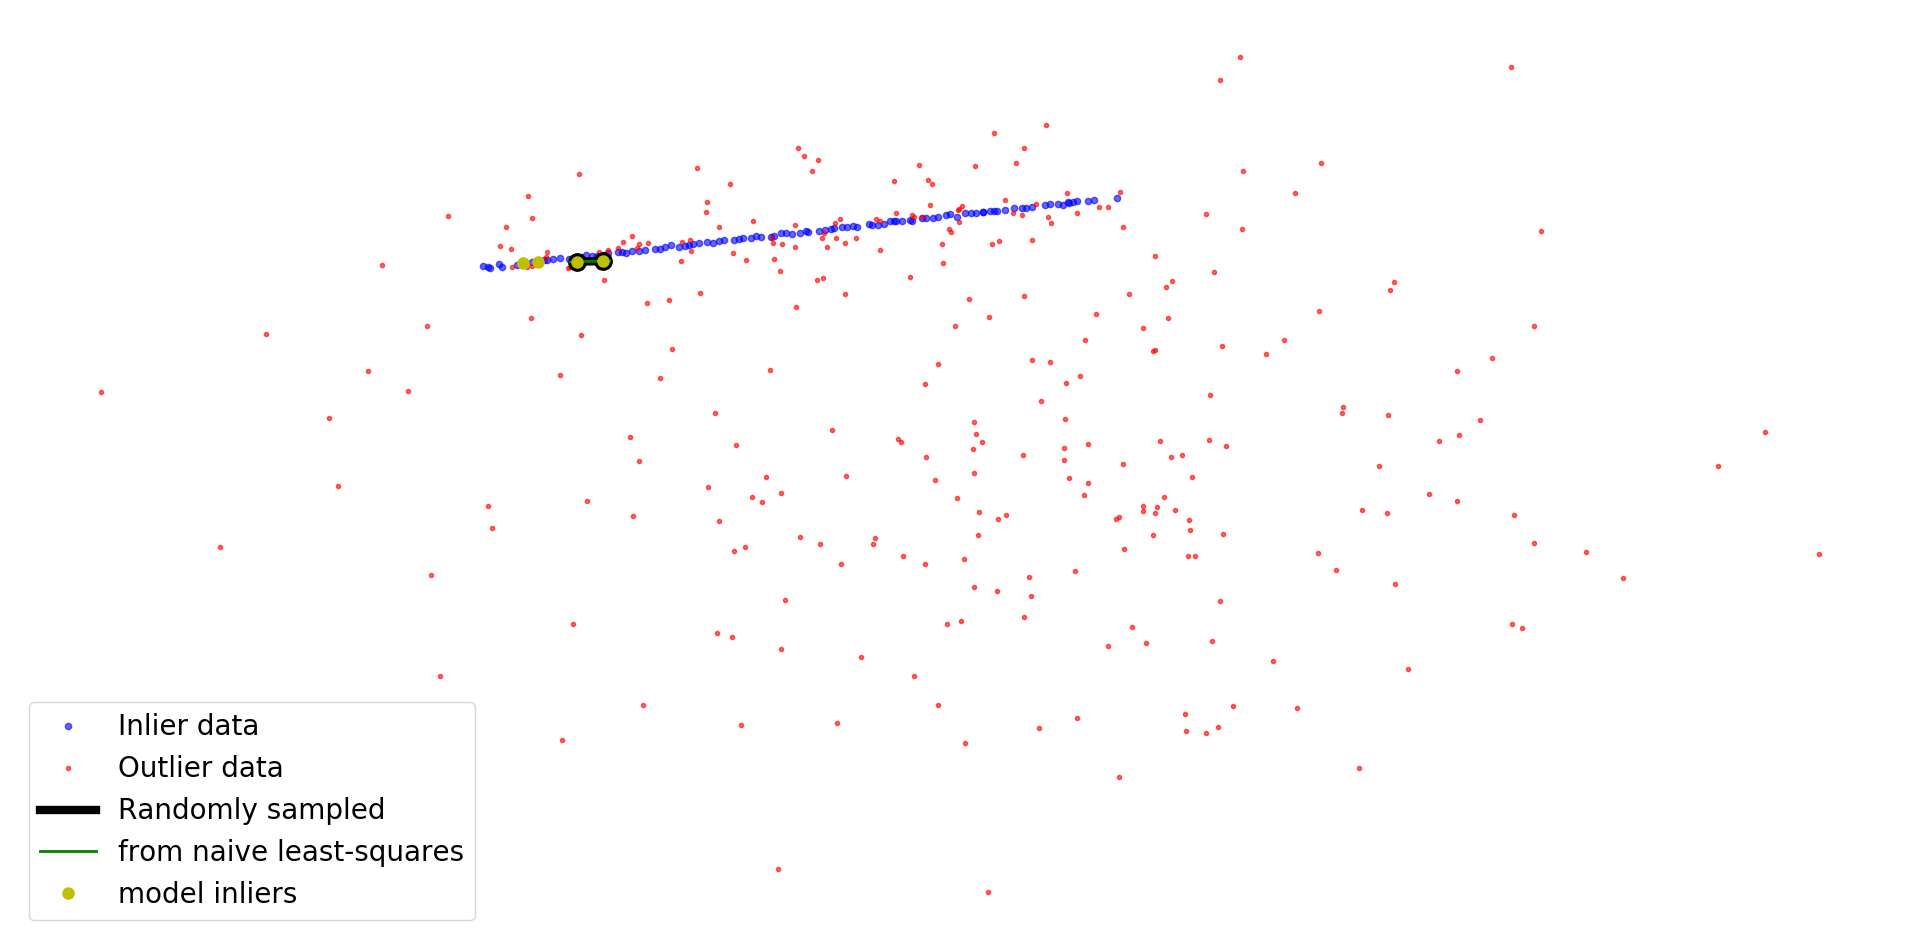
\includegraphics[width=0.95\textwidth]{FIGURES/ransac_trial_better}
  \end{center}
\end{frame}


\begin{frame}{Sample run in 2D: Getting C lose}
  \begin{center}
      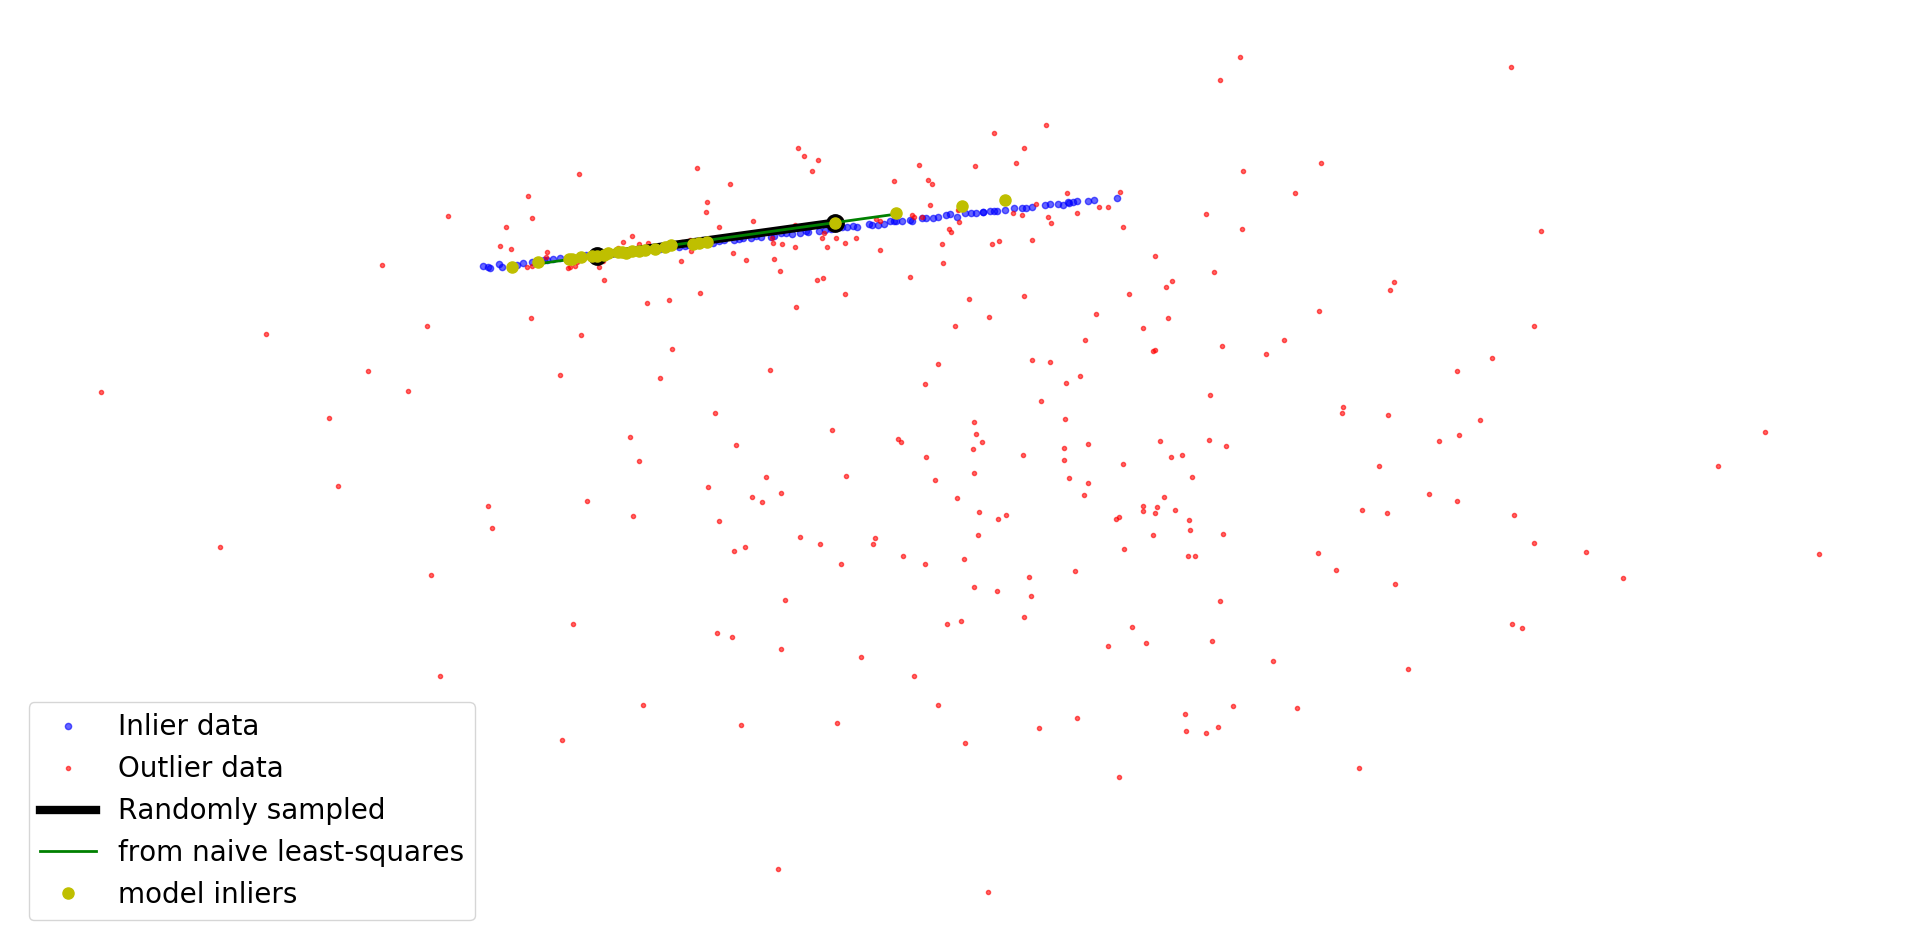
\includegraphics[width=0.95\textwidth]{FIGURES/ransac_trial_getting_close}
  \end{center}
\end{frame}


\begin{frame}{Sample run in 2D: Near Perfect}
  \begin{center}
      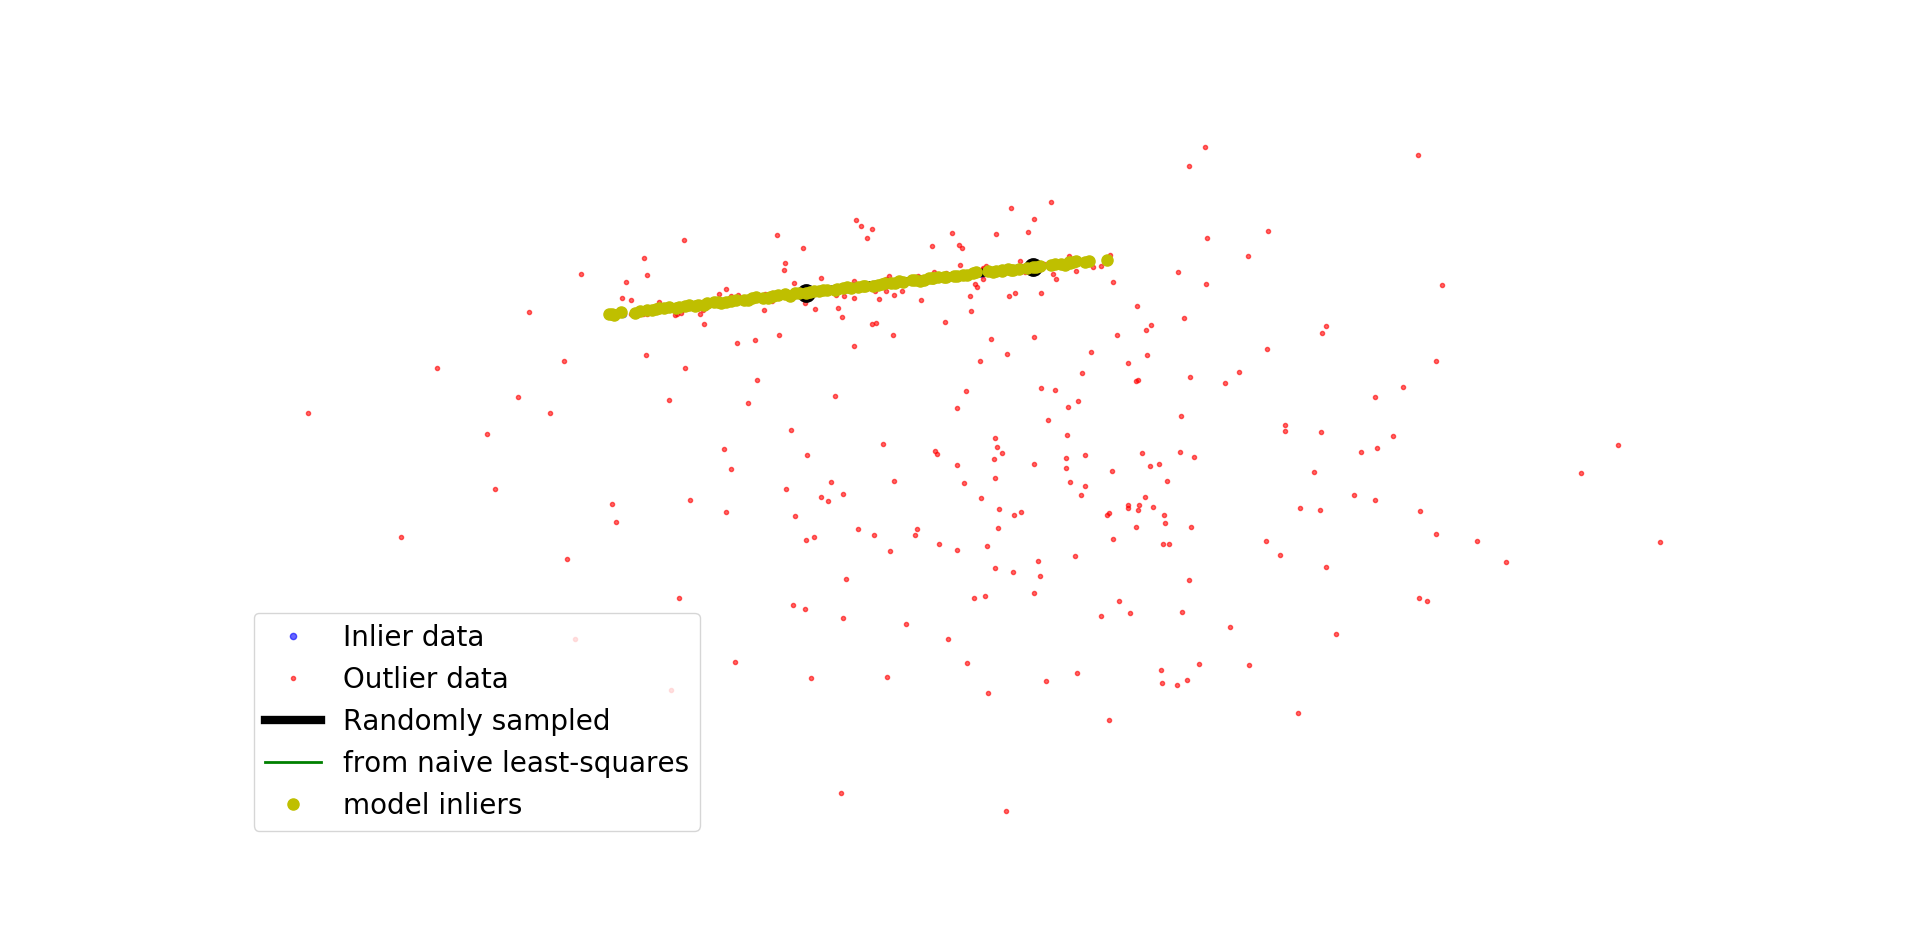
\includegraphics[width=0.95\textwidth]{FIGURES/ransac_trial_near_perfect}
  \end{center}
\end{frame}

\begin{frame}{How many trials}
  \vfill
  \begin{itemize}
  \item If model needs at least $n$ points to be fitted, can we guarantee that one can
    sample $n$ inliers at a given trial?\vfill
  \item Number of trial can be estimated from inlier frequency
    $$
    \text{inlier frequency } = \frac{\text{number of inliers}}{\text{total number of data points}}
    $$\vfill
  \item inlier frequency can be estimated from trial!\vfill
  \item Each trial reports a number of inlier for selected model.\vfill
  \item Take this number as lower bound for number of inliers.\vfill
  \end{itemize}
\end{frame}

\begin{frame}{How many trials}
  \begin{itemize}
  \item Fishler and Bolles show: Assume inlier frequency is $w$, and $n$ inliers are necessary to fit a model
  \item to be sure with probability $z$ that one can sample $n$ good points in a trial, number of trials $N$ at least
    $$
    N\approx\frac{\log(1-z)}{\log(1-w^n)}
    $$
  \item \dbend Depends critically on threshold for accepting / rejecting fits!
  \end{itemize}
\end{frame}


\begin{frame}{RANSAC and estimation of $\rho \bn = \bm$}
  \begin{itemize}[<+->]
  \item Data + Observation:
    \begin{itemize}
    \item $k$ light source vectors $s_1,\dots,s_k$
    \item Per pixel, $k$ intensity values $I_1(p),\dots I_k(p)$.
    \end{itemize}
  \item Relation between  model $\bm$ and observations: Lambert's law
    $$
    I_i(p)\approx s_i^T\bm(p)
    $$
  \item Minimal number of light vectors and corresponding measured intensities for
    determining a $\bm$?\uncover<6->{~~~~~~\myemph{3! (why?)}}\pause
  \item Can happen that 3 selected light vector are nearly colinear:\uncover<8->{ \myemph{Retry!}}\pause
  \item \myemph{NOTE:} One RANSAC must be run for \myemph{EACH} pixel! (Not as bad as it seems...)
  \item Good news: a special RANSAC \texttt{ransac\_3dvector()} for estimations of $\bm$ vectors is available from the \texttt{ps\_utils.py} module (Absalon).
  \end{itemize}
\end{frame}




\section{Normal Field Denoising}

\begin{frame}{Nice Normal Field. Good Integration}
  \begin{figure}[h]
    \centering
    \begin{tabular}[h]{c@{\hskip10mm}c}
      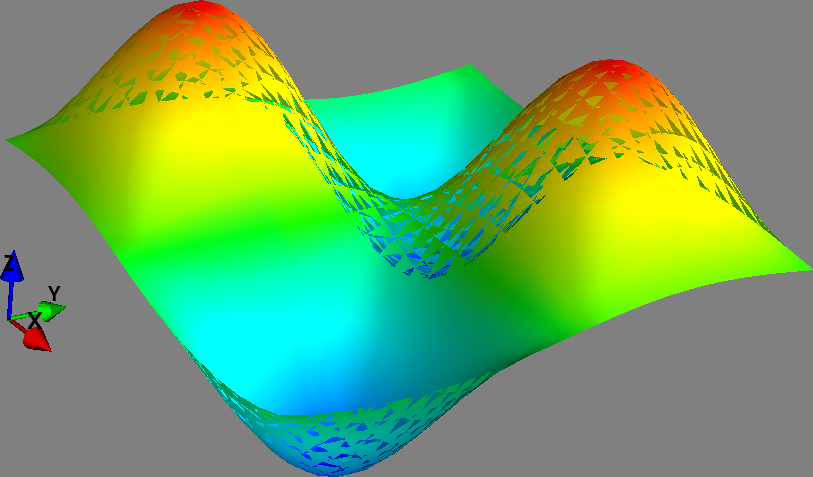
\includegraphics[width=0.4\textwidth,height=0.235\textwidth]{nfs/surface_gaussder11}&
      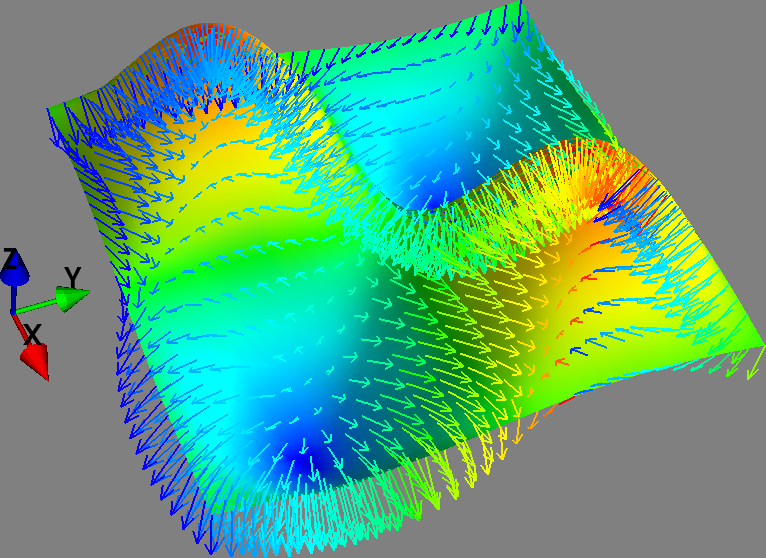
\includegraphics[width=0.4\textwidth,height=0.235\textwidth]{nfs/normalfield_gaussder11_onsurface}\\
      Original surface & With normal field plotted on it \\
      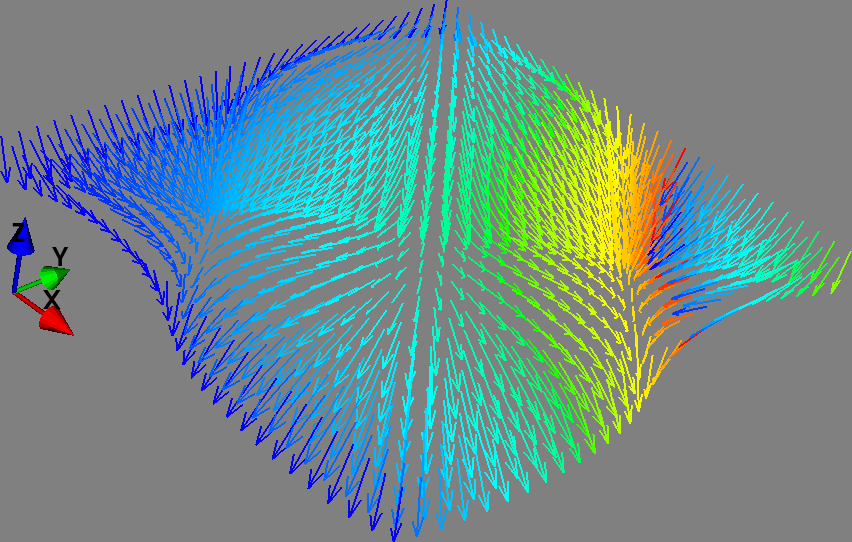
\includegraphics[width=0.4\textwidth,height=0.235\textwidth]{nfs/normalfield_gaussder11}&
      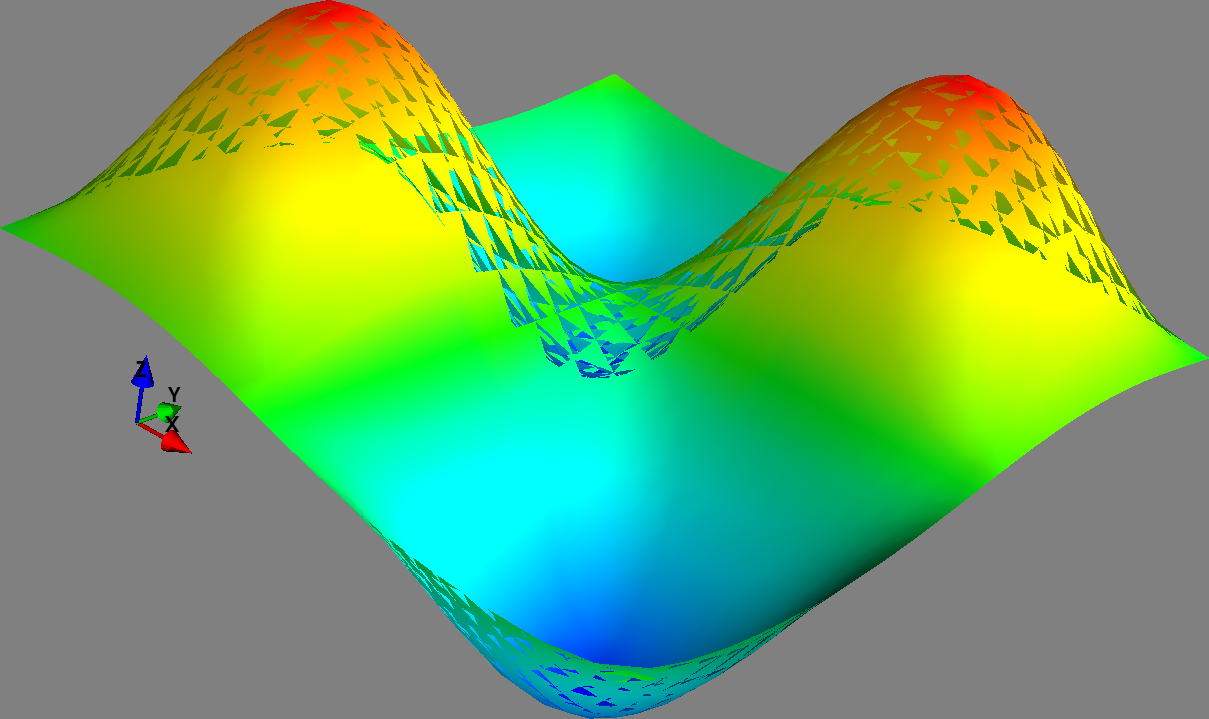
\includegraphics[width=0.4\textwidth,height=0.235\textwidth]{nfs/surface_from_integration_nf}\\
      Just the normal field & Numerical integration
    \end{tabular}
  \end{figure}
\end{frame}


\begin{frame}{Not So Nice Normal Field, Noisy Result}
  \begin{figure}[h]
    \centering
    \begin{tabular}[h]{c@{\hskip10mm}c}
      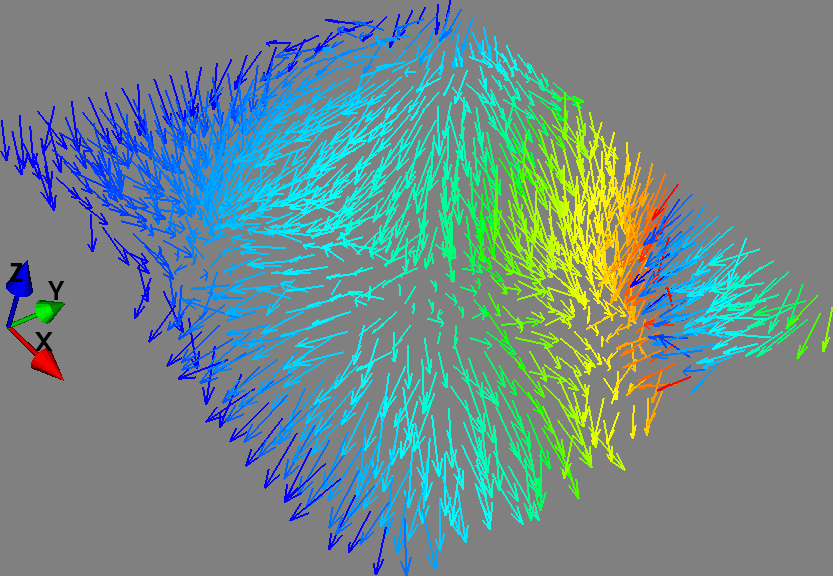
\includegraphics[width=0.4\textwidth,height=0.235\textwidth]{nfs/normalfield_gaussder11_noisy}&
      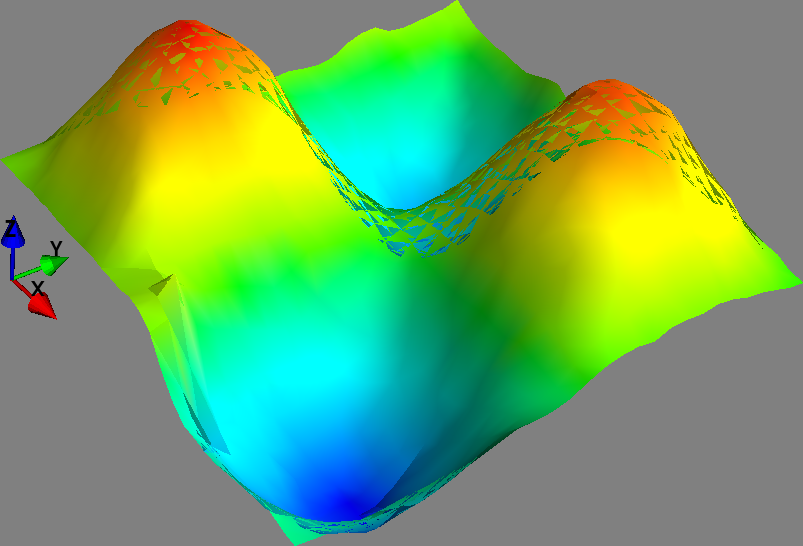
\includegraphics[width=0.4\textwidth,height=0.235\textwidth]{nfs/surface_from_integration_noisy_nf}\\
      Noisy normal field & Noisy surface recovery 
    \end{tabular}
  \end{figure}
  
\end{frame}


\begin{frame}{Noisy Vector field?. Denoising}
  \begin{figure}[h]
    \centering
    \begin{tabular}[h]{c@{\hskip20mm}c}
    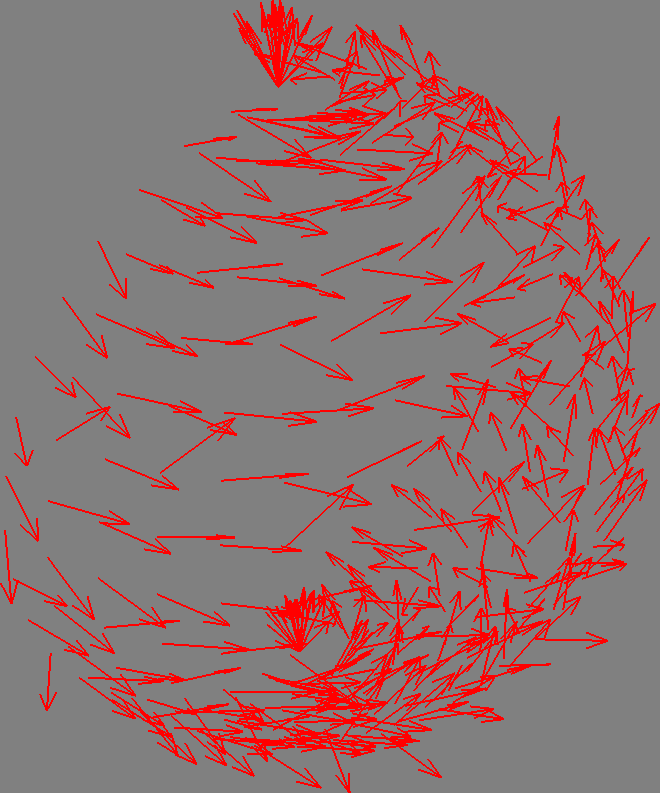
\includegraphics[width=0.3\textwidth]{FIGURES/noisy_field}&
    \uncover<2->{\includegraphics[width=0.3\textwidth]{FIGURES/denoised_field}}      
    \end{tabular}
  \end{figure}
  \pause
  \begin{itemize}
  \item Gaussian Convolution adapted to normal fields:
  \item each new vector value must still have norm 1.
  \item A bit complicated, uses differential geometry:-)
  \end{itemize}
  %A routine in \texttt{ps\_utils.py} module, \texttt{smooth\_normal\_field()} can do it. 
\end{frame}


\begin{frame}{Denoising and integration}
  \begin{figure}[h]
    \centering
    \begin{tabular}[h]{c@{\hskip3mm}c@{\hskip3mm}c}
      \includegraphics[width=0.3\textwidth,height=0.16\textwidth]{nfs/normalfield_gaussder11_noisy}&
      \includegraphics[width=0.3\textwidth,height=0.16\textwidth]{nfs/normalfield_gaussder11_noisy_denoised}&
      \includegraphics[width=0.3\textwidth,height=0.16\textwidth]{nfs/normalfield_gaussder11}\\
      Noisy normal field & Denoised field & Original clean 
    \end{tabular}
    \begin{center}
    \includegraphics[width=0.96\textwidth,height=0.3\textwidth]{nfs/integration_cleannf_vd_denoised_nf_vs_noisy_nf}  
    \end{center}
  \end{figure}
  \begin{itemize}
  \item In \texttt{ps\_utils.py} module, \texttt{smooth\_normal\_field()} can do it.
  \item For the assignment, keep its default parameters.
  \end{itemize}
  
\end{frame}

\section{Some examples}



\begin{frame}[t]{Process}
  \begin{center}
    \begin{tabular}[h]{cc}
      \includegraphics[width=0.3\textwidth]{FIGURES/Cat0} &
      \includegraphics[width=0.3\textwidth]{FIGURES/Catneedles}\\
      \includegraphics[width=0.3\textwidth]{FIGURES/CatAlbedo} &
      \includegraphics[width=0.3\textwidth]{FIGURES/cat_depth2}\\
    \end{tabular}
  \end{center}
  Top left: 1 of the input images, right: normal field. Bottom left: albedo, right: a 3D reconstruction.
\end{frame}



\begin{frame}[t]{Mezigue}
  \begin{center}
    \includegraphics[width=0.3\textwidth]{IMAGES/photometric_sample_all_jpg}
  \end{center}
  \begin{center}
    \begin{tabular}[h]{ccc}
      \onslide<2->{\includegraphics[width=0.3\textwidth]{IMAGES/photometric_sample_jpg_0001}} &
      \onslide<2->{ \includegraphics[width=0.3\textwidth]{IMAGES/photometric_sample_jpg_0006}} &
       \onslide<2->{\includegraphics[width=0.3\textwidth]{IMAGES/photometric_sample_jpg_0008}} 
    \end{tabular}
  \end{center}
  \begin{center}
    \onslide<3>{\includegraphics[width=0.15\textwidth]{IMAGES/point_cloud180}}
  \end{center}
\end{frame}


\begin{frame}{Literature, available in Abaslon}
  \begin{itemize}
  \item Horn, Shape from shading 1970
  \item Woodham, Photometric Stereo, 1980
  \item Fishler-Bolles, RANSAC, 1981
  \end{itemize}
  
\end{frame}


\begin{frame}[t]{Summary}
  \begin{itemize}
  \item \phos
  \item \metron
  \item \stereos
  \end{itemize}
  \begin{center}
    \only<2>{\includegraphics[width=0.3\textwidth]{FIGURES/Malescrunchedface-lrg}}
    \only<3>{\includegraphics[width=0.3\textwidth]{FIGURES/christmastree}}
  \end{center}
\end{frame}


\end{document}


% \section{Orthographic Camera}

% \begin{frame}[t]{Orthographic Camera}
%   \begin{center}%     \includegraphics[width=0.9\textwidth]{FIGURES/orthographic}
%   \end{center}
%   \begin{itemize}
%   \item Non physical: ``Camera at infinity'', parallel beams.
%   \item Projection Matrix:
%     $$
%     P =
%     \begin{bmatrix}
%       1 & 0 & 0\\
%       0 & 1 & 0
]%     \end{bmatrix}
%     $$
%   \item Useful for ``far objects''. In Some Transmission Imaging too, e.g. CT Scanning, Transmission Electron.Microscopy... 
%   \end{itemize}
% \end{frame}




% \begin{frame}
%   \frametitle{Multiple View Correspondences}
%   \begin{center}
%     \includegraphics[width=0.9\textwidth]{FIGURES/stereo}
%   \end{center}
%   If we can recover $x'$ from $x$ we can recover depth.
% \end{frame}

% \begin{frame}
%   \frametitle{Image Correspondence}
%   \begin{center}
%     \includegraphics[width=0.9\textwidth]{IMAGES/stereo2images}
%   \end{center}
%   How do we match points from image 1 to image 2: you should have seen some of it with Kim,
%   but this is not the end of the story!
% \end{frame}


% \begin{frame}
%   \frametitle{Epipolar Constraints}
%   \begin{center}
%     \includegraphics[width=0.9\textwidth]{FIGURES/epipolarconstraint}
%   \end{center}
%   \begin{itemize}
%   \item    Potential match for $x$ must lie in corresponding line $l'$
%   \item  Potential match for $x'$ must lie in corresponding line $l$
%   \end{itemize}  
% \end{frame}


% \begin{frame}
%   \frametitle{Epipolar Constraints}
%   \begin{center}
%     \includegraphics[width=0.9\textwidth]{FIGURES/epigeom}
%   \end{center}
%   \begin{itemize}
%   \item  Line connecting $O$ and $O'$: \myemph{baseline}
%   \item Plane through baseline $x$ and $x'$: \myemph{Epipolar Plane}
%   \item Epipoles: intersection of baseline and image planes:
%     projection of the other camera center.
%   \item Epipolar Lines - intersections of epipolar plane with image
%     planes (always come in corresponding pairs)
%   \end{itemize}  
% \end{frame}


% \begin{frame}
%   \frametitle{Example: Converging cameras}
%   \begin{center}
%      \includegraphics[width=0.9\textwidth]{FIGURES/convergecam}
%   \end{center}
% \end{frame}

% \begin{frame}
%   \frametitle{Calibrated Case}
%    \begin{center}
%     \includegraphics[width=0.65\textwidth]{FIGURES/epicalibrated}
%   \end{center}
%   Camera parameters known for the two cameras: calibration matrices $K$ and $K'$\\
% \end{frame}

% \begin{frame}
%   \begin{itemize}
%   \item  $x$ and $x'$ (in 3D coords but not the same)  are related by rotation and translation.
%     $$x' = R(x-\bt)$$
%   \item Their homogeneous coordinates $y$ and $y'$ are related by a simple matrix $E$ built from $R$ and $t$
%     $$
%     y^T E y = 0.
%     $$
%   \item $E$ is called the \myemph{essential matrix} (Longuet-Higgins 1981).
%   \item $E$ can be estimated from images.
%   \item The position and orientation of camera 1 vs camera 2 (i.e.,
%     $R$ and $\bt$) can be recovered from $E$.
%   \end{itemize}
% \end{frame}

% \begin{frame}
%   \frametitle{Note on the geometric transformation between image 1 and
%     image2}
%   \begin{itemize}
%   \item The transformation between $y$ and $y'$ is not linear: it is
%     an \myemph{homography} between the 2 image planes: 
%   \item An homography conserves straight lines, but not parallelism. 
%   \item Two parallel lines intersect at infinity: after an homography they may intersect at finite distance.
%   \end{itemize}
% \end{frame}


% \begin{frame}
%    \frametitle{Uncalibrated Case}
%    \begin{itemize}
%    \item No way to directly compare $x$ and $x'$: they relate through
%      the unknown transformations $K$ and $K'$.
%    \item A relation however still exists (Faugeras, Luong, 1992)
%      $$
%      y^T \udesc{F}{K^{-\top} E K'^{-1}} y =0
%      $$
%    \item $F$ is called the \myemph{fundamental matrix}. 
%    \item Though $K$ and $K'$ are unknown $F$ can be \myemph{esitimated}
%      (complicated) thus used for the correspondence problem!
%    \item {\small $K^\top$ is the transposed of $K$: inverse row and line indices.
%      For a vector in column, write it in line.}
%    \item {\small $K^{-1}$ is the inverse of $K$: provides the inverse change
%      of coordinates from unnormalized to normalized image coordinate.}
%    \item {\small $K^{-\top}$ means inverse of the transposed matrix: The same
%      as transposed of the inverse.}
%    \end{itemize}
% \end{frame}
